
\documentclass{article}
\usepackage[T1]{fontenc}
\usepackage[utf8]{inputenc}


% reference setting
\usepackage[colorlinks=true, citecolor=blue, linkcolor=blue, urlcolor=blue]{hyperref}
\usepackage{amsmath}
\usepackage{amssymb}
\usepackage{graphicx}
\usepackage{booktabs}

\usepackage[
  backend=biber,
  style=authoryear,
  maxcitenames=2,
  maxbibnames=99,
  giveninits=true
]{biblatex}

\addbibresource{mybibliography.bib}

% add comma before the year in parenthetical citations
\DeclareDelimFormat{nameyeardelim}{\addcomma\space}




% Adjust page margins
\usepackage{geometry}
\geometry{left=1.75in, right=1.75in, top=1.25in, bottom=1.25in}

% font
\usepackage{titlesec}
\titleformat{\section}{\normalfont\large\bfseries}{\thesection}{1em}{}
\titleformat{\subsection}{\normalfont\normalsize\bfseries}{\thesubsection}{1em}{}
\usepackage[font=footnotesize, labelfont=bf, margin=1cm]{caption}

% author
\usepackage{authblk}

% images
\graphicspath{ {./images/} }
\usepackage{subcaption}

% Proposition
\usepackage{amsthm}
\newtheorem{proposition}{Proposition}


\title{\textbf{Bayes Factor Testing of Linear and Nonlinear Effects in Additive Gaussian Process Regression}}
\author[1]{Yueheng Wu}
\author[2]{Joran Jongerling}
\author[3]{Joris Mulder}
\affil[1,2,3]{Department of Methodology and Statistics, Tilburg University}
\renewcommand\Authands{, }

\date{}

\begin{document}
\maketitle

\begin{abstract}
Gaussian process regression flexibly models nonlinear predictor--response relationships, but as a kernel-based nonparametric method it does not reveal whether a given predictor acts linearly, nonlinearly, or not at all. We propose a Bayesian testing framework for this problem within additive Gaussian process regression. Each predictor is decomposed into a linear component with a $g$-prior and an orthogonalized Gaussian process component capturing nonlinear structure beyond the linear trend; the latter is governed by a standardized magnitude parameter whose value zero removes the component, yielding a scalar null hypothesis for nonlinearity. Linear and nonlinear effects are assessed separately through Bayes factors computed from a single posterior simulation of the full model via Savage--Dickey-type identities, so that no separate null and alternative models need be fit. For nonlinear effects we introduce an interval-null Bayes factor based on the encompassing-prior generalization of the Savage--Dickey ratio, which applies under both local and non-local priors and converges to the point-null Bayes factor as the interval shrinks, with bridge sampling as an independent benchmark. Simulations and applications to four benchmark datasets show that the method reliably distinguishes linear, nonlinear, and negligible effects.
\end{abstract}


\section{Introduction}

Many empirical relationships are not well described by a straight line, so identifying and characterizing nonlinear effects is a recurring problem in applied research. Linear regression remains a standard tool because its coefficients are easy to interpret and its inferential properties are well understood. Nonlinear patterns can be incorporated within the linear modeling framework through pre-specified basis expansions, such as polynomial terms or regression splines \parencite{stone1997use}, but these approaches require the researcher to choose a functional form in advance. More flexible approaches relax this requirement to varying degrees: generalized additive models estimate smooth predictor contributions from the data \parencite{hastie1990generalized}, whereas kernel-based methods provide another route by defining similarity between observations through a kernel \parencite{scholkopf2001learning}.

Gaussian process (GP) regression \parencite{williams2006gaussian} provides a kernel-based framework for representing unknown relationships between predictors and a response. Rather than fixing a parametric form, a Gaussian process places a prior directly on the function relating predictors to the response, with smoothness assumptions encoded through a covariance kernel \parencite{Williams1996}. The data then inform the shape of the fitted function, while the resulting uncertainty quantification reflects what remains unresolved after observing the data. This makes GP regression a flexible alternative when the form of the predictor--response relationship is not known in advance.

Despite its flexibility, GP regression does not directly reveal how each predictor contributes to the response. The earliest approach to this problem, automatic relevance determination (ARD), uses predictor-specific length-scale parameters as a proxy for relevance \parencite{mackay1992bayesian, neal1995bayesian}: a large length-scale is interpreted as indicating low influence on the response. Length-scales, however, primarily control the smoothness of the fitted function rather than the strength of association, and a predictor with little influence can still be associated with a small length-scale \parencite{linkletter2006variable, nakajima2007theoretical, piironen2016projection}. A more fundamental difficulty is that linear and nonlinear contributions are not separated within standard GP inference. \textcite{gramacyGaussianProcessesLimiting2008} showed that the linear model is a limiting special case of the GP, yet standard GP priors assign negligible posterior probability to this limit even when the data are genuinely linear, so a fitted GP conflates the two types of structure. This motivates an approach that makes the separation explicit. The goal of the present paper is to separately assess, for each predictor, whether it contributes no effect, a linear effect, or a nonlinear departure from linearity. Several existing strategies bear on this goal, but each stops short of a formal test.

Sensitivity analysis and projection-based variable selection assess predictor influence by measuring predictive change. Sensitivity-based approaches summarize how much the posterior predictive distribution changes when an input is perturbed, either globally over the input domain by attributing model-output variation to individual predictors or their interactions \parencite{oakley2004probabilistic}, or locally near the observed data \parencite{paananen2019variable}. Projection-based methods instead fit a reference model on all predictors and then identify reduced models whose predictive distributions remain close to that reference \parencite{piironen2016projection}. Both families describe predictive influence, but their target is predictive change or fidelity rather than evidence for a null hypothesis.

Bayesian sparsity priors address variable selection more directly by encoding inclusion decisions within the prior \parencite{mitchell1988bayesian, george1993variable}. In GP models, this can be achieved with spike-and-slab formulations or binary inclusion indicators on inputs, kernel parameters, or covariance components \parencite{linkletter2006variable, savitsky2011, titsias2011spike}, which assign posterior probability to whether a predictor or component is active. These approaches are closer to inferential variable selection than sensitivity or projection methods, but posterior inclusion probabilities do not by themselves quantify the evidence that a given component is supported by the data in the sense of a formal hypothesis test.

Kernel design strategies pursue interpretability by decomposing the covariance function into structured components corresponding to main effects and interactions, as in additive and functional-ANOVA kernel constructions \parencite{duvenaud2011a, durrande2013anova}. Structure-discovery approaches extend this idea by searching over sums and products of kernels to obtain expressive but interpretable covariance structures \parencite{duvenaud2013structure}, and hierarchical priors or kernel-weighting schemes can encourage sparsity across components \parencite{archambeau2011multiple}. These methods help represent and organize linear and nonlinear structure, but representation is not the same as testing: deciding whether a given component is supported by the data still requires a principled inferential criterion, and the additional kernel choices, component-specific hyperparameters, and model-search uncertainty complicate that assessment.

Bayes factors address this inferential gap by comparing the marginal probabilities of competing models and quantifying the evidence they contain while penalizing unnecessary complexity \parencite{kass1995bayes, jeffreys1961theory}. Marginal likelihoods for GP regression are analytically intractable, and although Bayes factors for GP models have been studied \parencite{mukhopadhyay2021}, their practical use has been limited by the difficulty of evaluating marginal likelihoods in non-conjugate settings.

In a related contribution, \textcite{mulder2023} applies Bayes factors to quantify evidence for the degree of nonlinearity in a single-predictor setting. Building on this evidence-based perspective, the present paper targets the presence of nonlinear contributions through a predictor-specific magnitude parameter in a multi-predictor additive GP model. For each predictor, the model contains a linear component and a nonlinear Gaussian process component constructed to be orthogonal to the linear space \parencite{PlumleeJoseph2018}, so that the nonlinear component captures only structure not already represented by the linear trend. The magnitude of each nonlinear component is controlled by a scalar parameter defined on a standardized scale: when this parameter is zero, the corresponding nonlinear contribution vanishes regardless of the smoothness of the underlying Gaussian process, so that testing whether a nonlinear effect is present reduces to testing whether this magnitude parameter is zero.

Priors on the magnitude parameters are calibrated on this standardized scale to reflect plausible ranges of nonlinear departure. In addition to this default local prior, we consider a non-local specification \parencite{johnson2010nonlocal} as an alternative that forces the prior density to vanish at the null and thereby sharpens the separation between the null and alternative hypotheses. Evidence for each linear effect, and separately for each nonlinear effect, is quantified through Bayes factors obtained via the Savage--Dickey density ratio and its encompassing-prior extension \parencite{Dickey1971, verdinelli1995, wetzels2010encompassing, mulder2022generalization}, each requiring only a single fit of the full model; bridge sampling \parencite{Meng1996, Gronau2017} is used as an independent benchmark. The behavior of the procedure is examined through a simulation study, and its practical use is illustrated on real datasets with comparison to findings from previous analyses.

The remainder of the paper is organized as follows. Section~\ref{sec:model} develops the additive decomposition of each predictor into orthogonal linear and nonlinear components and the associated hypothesis tests. Section~\ref{sec:priors} specifies the priors on the magnitude parameters and describes how the linear and nonlinear Bayes factors are computed from a single model fit. Section~\ref{sec:simulation} reports a simulation study, and Section~\ref{sec:empirical} illustrates the method on four datasets. Section~\ref{sec:discussion} concludes.

%%% ============================================================
%%%  SECTION 2 — MODEL
%%% ============================================================
\section{Modeling framework\label{sec:model}}

Let $\mathbf{y}\in\mathbb{R}^n$ denote a vector of $n$
observations of the response variable $Y$, and let
$\mathbf{X}\in\mathbb{R}^{n\times(p+1)}$ be the full-rank design matrix
containing the intercept and $p$ candidate predictors.
We model the relationship between predictors and the response through
an additive decomposition of linear and nonlinear contributions:
%
\begin{align}
\label{eq:model}
\mathbf{y}
  &= \sigma\,\mathbf{X}\boldsymbol{\theta}
   \;+\; \sum_{j=1}^{p}\mathbf{f}_j
   \;+\; \boldsymbol{\varepsilon},
\\
\label{eq:prior-theta}
&\theta_0 \sim \mathcal{N}\!\bigl(0,\; v_0\bigr),
\qquad
\boldsymbol{\theta}_{1:p}\mid g
  \sim \mathcal{N}\!\bigl(\mathbf{0},\;
       g\,(\mathbf{X}_{p}^{\!\top}\mathbf{X}_{p})^{-1}\bigr), 
\\
\label{eq:prior-fj}
&\mathbf{f}_j \mid \delta_j,\lambda_j
  \sim \mathcal{N}\!\bigl(\mathbf{0},\;
       \sigma^2\,\delta_j^{\,2}\,\widetilde{\mathbf{K}}_j\bigr),
\\
&\boldsymbol{\varepsilon}
  \sim \mathcal{N}(\mathbf{0},\,\sigma^2\mathbf{I}_n).
\end{align}

Here, $\boldsymbol{\theta} = [\theta_0, \theta_1, \dots, \theta_p]^\top$ collects the intercept~$\theta_0$ and the standardized linear coefficients $\boldsymbol{\theta}_{1:p}=(\theta_1,\dots,\theta_p)^\top$,
each $\mathbf{f}_j\in\mathbb{R}^n$ is a latent nonlinear component
associated with predictor $j$, and $\boldsymbol{\varepsilon}$ is a
Gaussian error term with unknown variance $\sigma^2$.
The scalar $g>0$ controls the shrinkage of the linear coefficients,
each $\delta_j\ge 0$ measures the magnitude of the $j$th nonlinear
departure from linearity, and each $\lambda_j>0$ controls the smoothness
of the corresponding nonlinear component.
The matrix $\widetilde{\mathbf{K}}_j$ is the orthogonalized kernel
matrix defined in \eqref{eq:ortho-kernel} below.
The common scale factor $\sigma$ ensures that both
$\theta_j$ and $\delta_j$ are expressed on standardized scales.


\subsection{Linear component: \texorpdfstring{$g$}{g}-prior\label{subsec:linear}}

The prior on the predictor coefficients $\boldsymbol{\theta}_{1:p}$ in
\eqref{eq:prior-theta} is Zellner's $g$-prior
\parencite{Zellner1986}, a standard construction in Bayesian regression.
Here $\mathbf{X}_p$ denotes the $n\times p$ submatrix of predictor columns,
i.e.\ the design matrix $\mathbf{X}$ without its intercept column.
The $g$-prior scales the covariance of $\boldsymbol{\theta}_{1:p}$ by
$(\mathbf{X}_p^{\!\top}\mathbf{X}_p)^{-1}$, so that the prior adapts to
the correlation structure and geometry of the predictors
\parencite{Liang2008, Rouder2012}.
The hyperparameter $g$ determines the overall amount of shrinkage:
small values pull the linear coefficients toward zero, whereas large
values yield weaker shrinkage.
The intercept $\theta_0$ is excluded from the $g$-prior and instead
receives a wide, weakly informative prior $\mathcal{N}(0,v_0)$ with a
large fixed variance $v_0$, so that it is left effectively unshrunk.


\subsection{Nonlinear component: orthogonalized Gaussian process prior
\label{subsec:gp}}

To represent nonlinear effects, we place a Gaussian process prior
on each latent function $f_j(\cdot)$ and let
$\mathbf{f}_j = \bigl(f_j(x_{1j}),\dots,f_j(x_{nj})\bigr)^\top$
denote its realization at the observed values of predictor $j$.
A GP is fully characterized by a mean function and a covariance kernel:
the mean function describes the prior average trend, whereas the kernel
determines how strongly function values at two input locations are
expected to co-vary.
In the present model, we set the GP mean function to zero because the
intercept and linear effects are already represented explicitly by the
regression component $\sigma\mathbf{X}\boldsymbol{\theta}$.

For each predictor $j$, we use the squared exponential kernel
%
\begin{equation}
\label{eq:se-kernel}
k_j(x,x'\mid\lambda_j)
  = \exp\!\left(
      -\frac{(x-x')^2}{2\lambda_j^2}
    \right),
\end{equation}
%
which satisfies $k_j(x,x)=1$.
%

This kernel implies smooth sample paths: larger $\lambda_j$ produces
more slowly varying nonlinear trends, whereas smaller $\lambda_j$
allows more local variation.
The corresponding kernel matrix $\mathbf{K}_j$ is obtained by evaluating
$k_j(\cdot,\cdot\mid\lambda_j)$ at all observed pairs of predictor
values. Other kernels, such as those from the Mat\'ern class, could be
used when rougher sample paths are substantively more appropriate. In
our specification, the covariance of the nonlinear component is
$\sigma^2 \delta_j^2 \mathbf{K}_j$, so the two GP hyperparameters play
distinct roles: $\lambda_j$ controls the smoothness of the function
through the kernel, whereas $\delta_j$ controls the overall magnitude of
the nonlinear component. Because this magnitude is expressed relative to
the noise scale $\sigma$, $\delta_j$ has a standardized interpretation
as the GP marginal standard deviation relative to the residual standard
deviation (before orthogonalization; the projection in
\eqref{eq:ortho-kernel} reduces the realized magnitude somewhat).

A key difficulty is that the GP terms can absorb variation that is
already explained by the linear predictor, because smooth GP
realizations can themselves exhibit broad trends over the observed
predictor range, and with large $\lambda_j$ these trends can be close
to linear.
This creates confounding between the linear and nonlinear parts of the
model and makes the decomposition hard to interpret.
Following \textcite{PlumleeJoseph2018}, we therefore orthogonalize each
kernel with respect to the column space of the full design matrix
$\mathbf{X}$, that is, against the intercept and every linear term
jointly.
Let
%
\begin{equation}
\label{eq:projection}
\mathbf{P}
  = \mathbf{X}(\mathbf{X}^{\!\top}\mathbf{X})^{-1}\mathbf{X}^{\!\top}
\end{equation}
%
be the projection matrix onto $\operatorname{col}(\mathbf{X})$.
We then define the orthogonalized kernel matrix
%
\begin{equation}
\label{eq:ortho-kernel}
\widetilde{\mathbf{K}}_j
  = (\mathbf{I}_n-\mathbf{P})\mathbf{K}_j(\mathbf{I}_n-\mathbf{P}).
\end{equation}
%
This construction ensures that the nonlinear component is orthogonal
to the linear predictor space, so that the GP captures only structure
not already represented by the intercept and linear trend.

We can see the roles of the two GP
hyperparameters from Figure~\ref{fig:gp_effects}.
As $\delta_j$ decreases toward zero, the nonlinear contribution
vanishes regardless of the value of $\lambda_j$.
The magnitude parameter therefore acts as the
presence--absence parameter for nonlinear structure.
This distinction also clarifies a limitation of ARD based solely on
length-scales: length-scales describe
the smoothness of an effect, but do not by themselves provide a clean
measure of whether the nonlinear effect is present.

\begin{figure}[ht] \centering 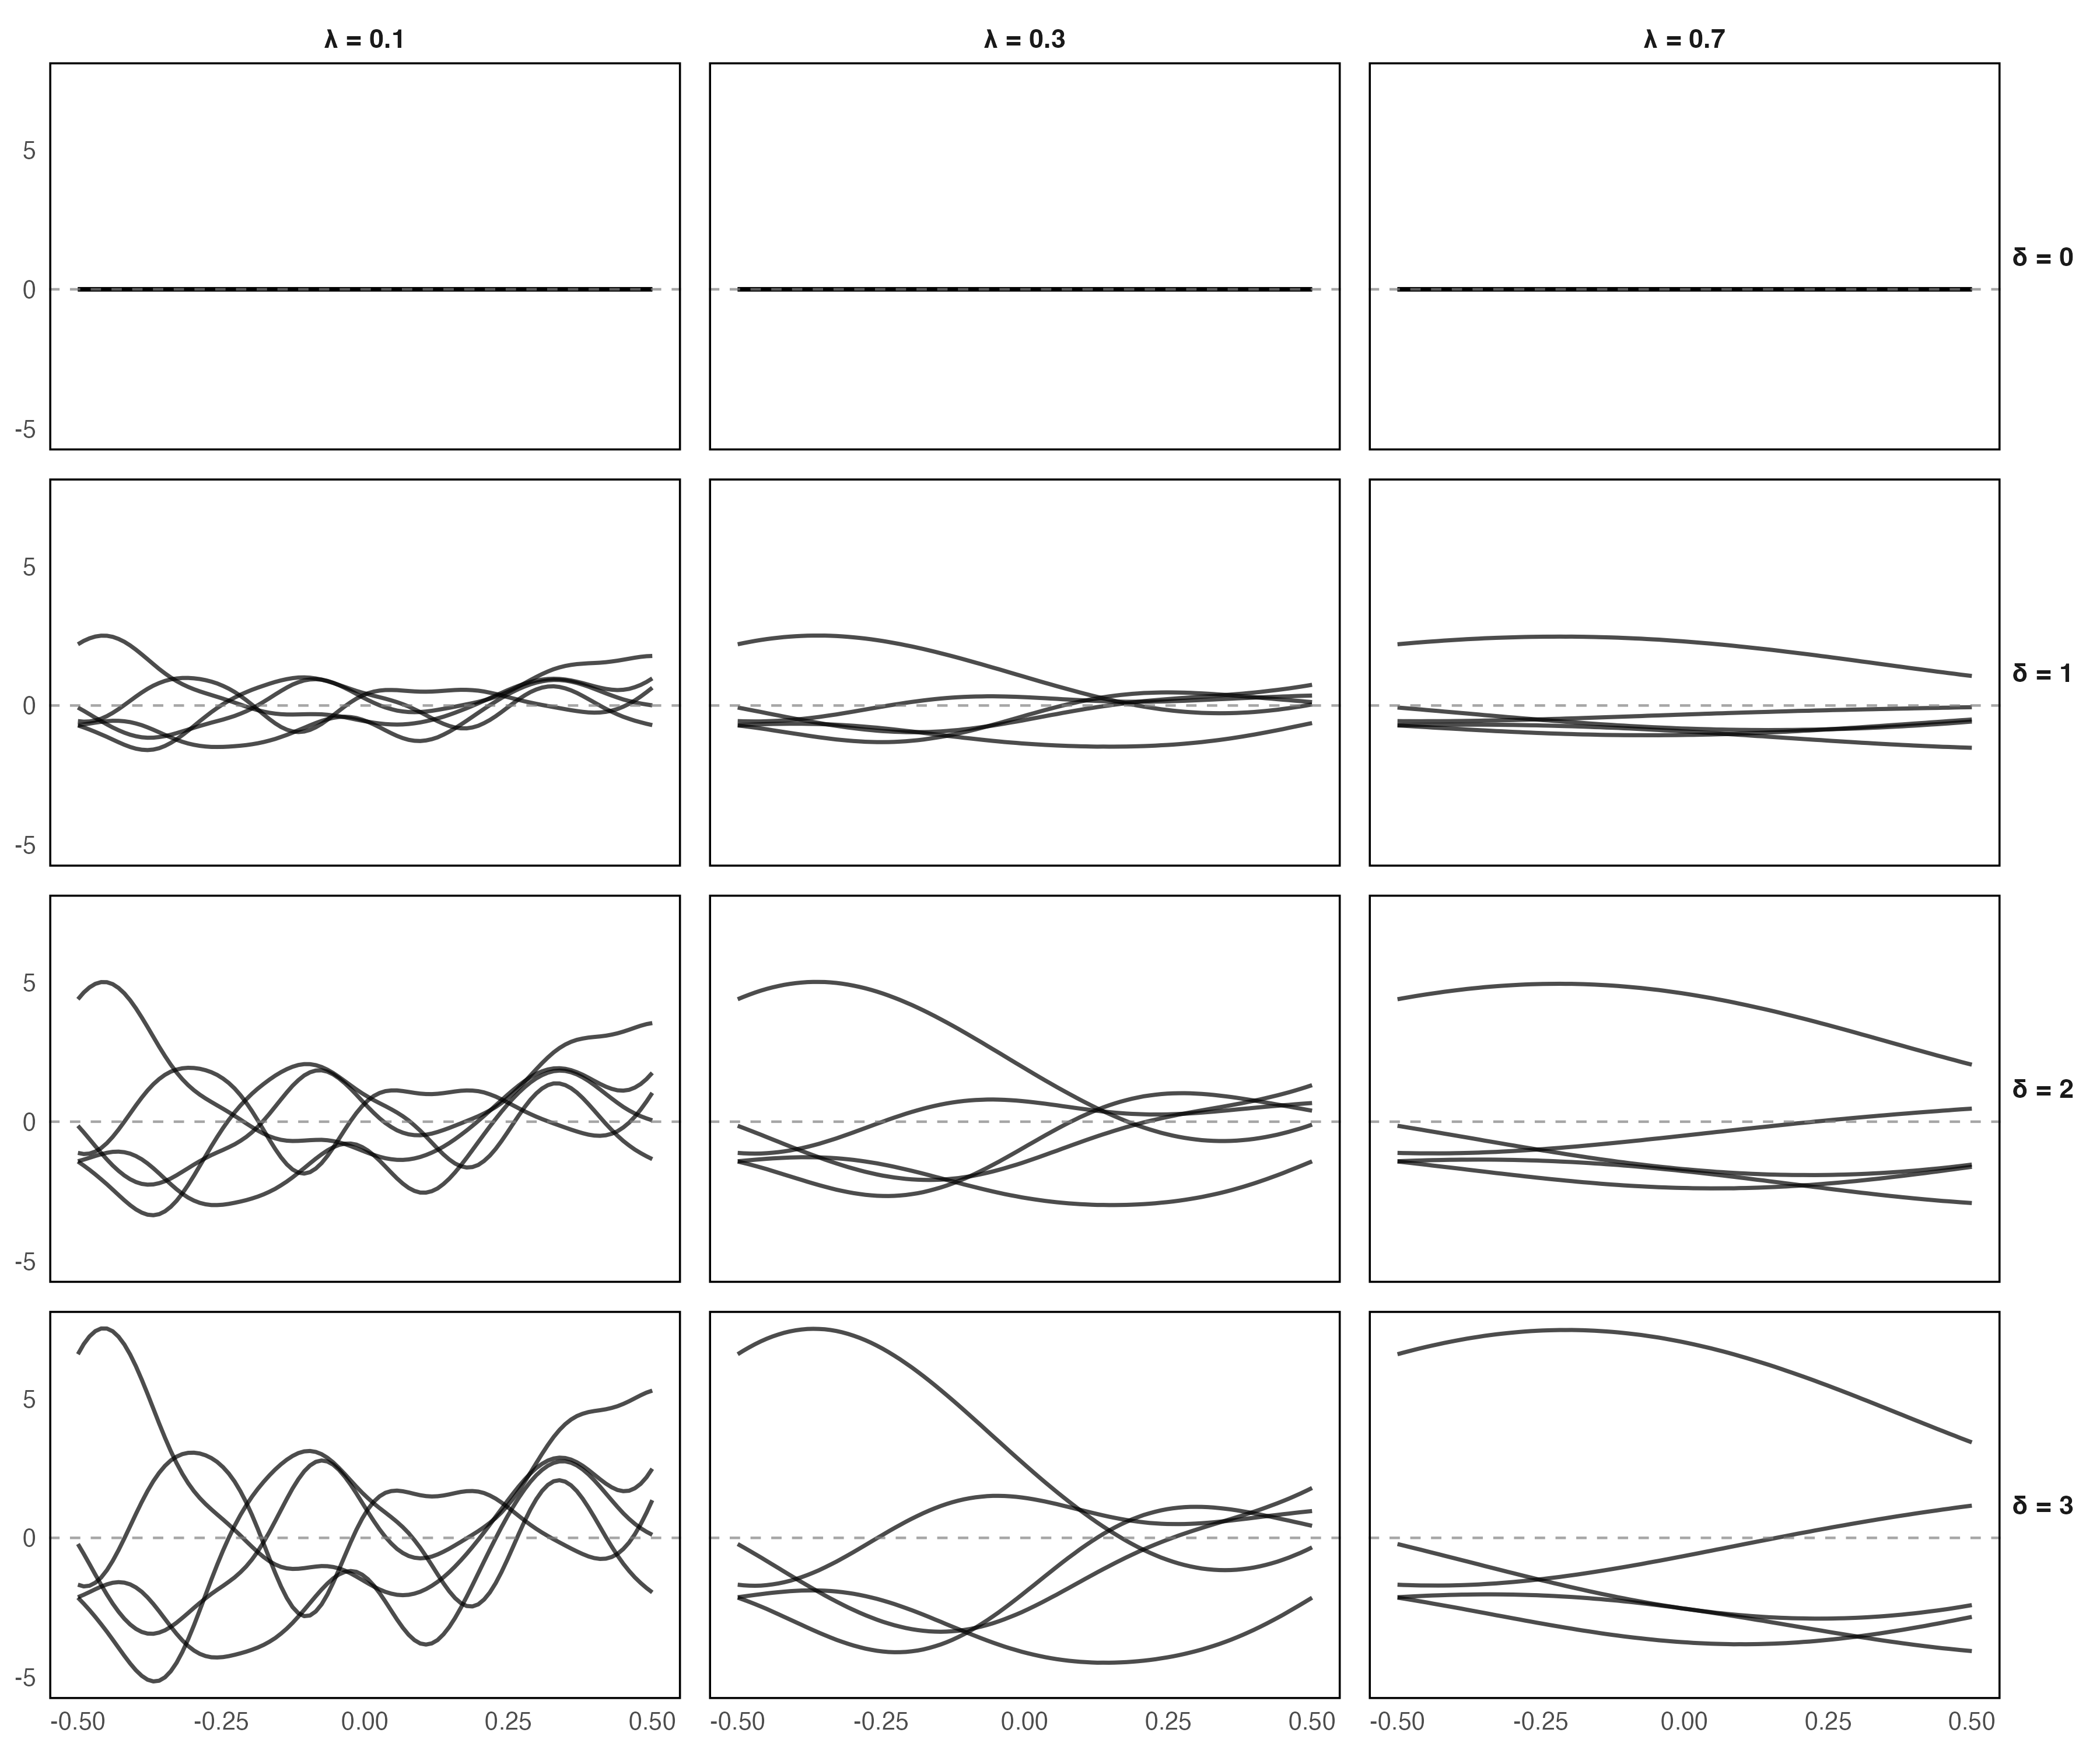
\includegraphics[width=1\textwidth]{images/plot-2-1.png} \caption{Gaussian-process realizations for selected values of the standardized nonlinear magnitude \(\delta\) and length-scale \(\lambda\), with predictor range fixed at 1. Nonlinearity increases as \(\delta\) grows and \(\lambda\) decreases. When \(\delta=0\), the GP contributes no nonlinear effect irrespective of \(\lambda\).} \label{fig:gp_effects} \end{figure}


\subsection{Marginal sampling distribution\label{subsec:marginal}}

Because the latent vectors $\mathbf{f}_1,\dots,\mathbf{f}_p$ are
Gaussian, they can be integrated out analytically.
This yields a marginal sampling distribution under the full model,
which contains both the linear component and all additive nonlinear
components:
%
\begin{equation}
\label{eq:marginal}
M_1:\quad
\mathbf{y}\mid\sigma^2,\boldsymbol{\theta},
\boldsymbol{\delta},\boldsymbol{\lambda}
\;\sim\;
\mathcal{N}\!\Bigl(
  \sigma\,\mathbf{X}\boldsymbol{\theta},\;
  \sigma^2\mathbf{I}_n
  + \sigma^2\sum_{j=1}^{p}\delta_j^{\,2}\widetilde{\mathbf{K}}_j
\Bigr),
\end{equation}
%
where $\boldsymbol{\delta}=(\delta_1,\dots,\delta_p)$ and
$\boldsymbol{\lambda}=(\lambda_1,\dots,\lambda_p)$.

This marginalized form is convenient because it avoids explicit
sampling of the high-dimensional latent functions while remaining
equivalent, for inference on $\mathbf{y}$, to the hierarchical
representation in \eqref{eq:model}--\eqref{eq:prior-fj}.
Beyond this computational convenience, the marginalized form is also
the object on which the hypothesis tests of
Section~\ref{subsec:testing} operate.


\subsection{Hypothesis testing\label{subsec:testing}}

For each predictor, we consider two inferential questions: whether its linear coefficient should be retained, and whether its nonlinear component should be included.

To test the linear effect of predictor $j$, we compare the full model
against a restricted model in which the $j$th linear coefficient is
removed:
%
\begin{equation}
\label{eq:model-minus-theta-j}
M_{0,j}^{(L)}:\quad
\mathbf{y}\mid\sigma^2,\boldsymbol{\theta}_{-j},
\boldsymbol{\delta},\boldsymbol{\lambda}
\;\sim\;
\mathcal{N}\!\Bigl(
  \sigma\,\mathbf{X}_{-j}\boldsymbol{\theta}_{-j},\;
  \sigma^2\mathbf{I}_n
  + \sigma^2\sum_{l=1}^{p}\delta_l^{\,2}\widetilde{\mathbf{K}}_l
\Bigr),
\end{equation}
%
which corresponds to testing
%
\begin{equation}
\label{eq:test-linear}
H_{0,j}^{(L)}:\;\theta_j = 0
\qquad\text{versus}\qquad
H_{1,j}^{(L)}:\;\theta_j \neq 0.
\end{equation}

To test the nonlinear effect of predictor $j$, we compare the full
model against a restricted model in which the $j$th nonlinear
component is removed:
%
\begin{equation}
\label{eq:model-minus-delta-j}
M_{0,j}^{(N)}:\quad
\mathbf{y}\mid\sigma^2,\boldsymbol{\theta},
\boldsymbol{\delta}_{-j},\boldsymbol{\lambda}_{-j}
\;\sim\;
\mathcal{N}\!\Bigl(
  \sigma\,\mathbf{X}\boldsymbol{\theta},\;
  \sigma^2\mathbf{I}_n
  + \sigma^2\sum_{l\neq j}\delta_l^{\,2}\widetilde{\mathbf{K}}_l
\Bigr),
\end{equation}
%
which corresponds to testing
%
\begin{equation}
\label{eq:test-nonlinear}
H_{0,j}^{(N)}:\;\delta_j = 0
\qquad\text{versus}\qquad
H_{1,j}^{(N)}:\;\delta_j > 0.
\end{equation}

The corresponding Bayes factors and their computation are developed
in Section~\ref{sec:priors}.


%%% ============================================================
%%%  SECTION 3 — PRIORS AND BAYES FACTOR COMPUTATION
%%% ============================================================
\section{Prior specification and Bayes factor
  computation\label{sec:priors}}

This section first specifies the hyperpriors on
$g$, $\boldsymbol{\delta}$, and $\boldsymbol{\lambda}$
(Section~\ref{subsec:prior-spec}), then defines the Bayes factor as
the evidence measure for the tests in
\eqref{eq:test-linear} and \eqref{eq:test-nonlinear}, and finally describes
the computational methods used to evaluate or approximate it
(Section~\ref{subsec:bf-computation}).


\subsection{Prior specification\label{subsec:prior-spec}}


\subsubsection{Prior on \texorpdfstring{$g$}{g}\label{subsubsec:prior-g}}
 
We assign an inverse-gamma hyperprior to the shrinkage parameter:
%
\begin{equation}
\label{eq:prior-g}
g \;\sim\; \mathrm{IG}\!\bigl(a = 2,\; b = \tfrac{n}{2}\bigr).
\end{equation}
%
Under this specification the marginal prior for each standardized
coefficient, obtained by integrating out~$g$, is a scaled
$t$-distribution,
%
\begin{equation}
\label{eq:marginal-theta}
\theta_j \;\sim\; t\!\bigl(2a,\; 0,\;
  \sqrt{b\,v_j / a}\bigr),
  \qquad v_j = \bigl[(\mathbf{X}_p^{\top}\!\mathbf{X}_p)^{-1}\bigr]_{jj},
\end{equation}
%
which for $a=2$ and $b=n/2$ gives $\theta_j \sim t(4,\,0,\,
\sqrt{n\,v_j/4})$.
The scale $b=n/2$ is the Zellner--Siow scale
\parencite{ZellnerSiow1980, Liang2008}, which ties the prior on $g$ to
the sample size so that the shrinkage induced on
$\boldsymbol{\theta}_{1:p}$ remains stable as $n$ grows.
Because the linear coefficients enter the model on the standardized
scale through the term $\sigma\,\mathbf{X}\boldsymbol{\theta}$ in
\eqref{eq:model}, the resulting Bayes factors for linear effects are
invariant to linear rescaling of both predictors and the response
\parencite{Rouder2012}.
 
This specification belongs to the family of mixture-of-$g$ priors
studied by \textcite{Liang2008}, who note that the classical
Zellner--Siow Cauchy prior \parencite{ZellnerSiow1980}, $g \sim \mathrm{IG}(1/2,\, n/2)$, does not
permit closed-form marginal likelihoods, limiting its adoption in
practice.
In our joint linear--GP model the problem is more severe: the
$\mathrm{IG}(1/2,\, n/2)$ density has a pole at $g = 0$, which
produces divergent transitions in Hamiltonian Monte Carlo sampling.
Setting $a = 2$ eliminates this pole, yields a proper prior with a
finite-variance $t(4)$ marginal on~$\boldsymbol{\theta}$, and
satisfies the model-selection desiderata of
\textcite{Bayarri2012}.

\subsubsection{Prior on \texorpdfstring{$\delta_j$}{delta j}\label{subsubsec:prior-delta}}

The standardized GP magnitude $\delta_j$ controls the presence and
strength of the $j$th nonlinear effect. Because $\delta_j$ is the ratio
of the GP marginal standard deviation to the noise standard deviation,
it has a direct signal-to-noise interpretation. This interpretation is shared
across predictors, which allows the prior on $\delta_j$ to be calibrated
on a common and substantively interpretable scale. The prior on $\delta_j$ therefore
serves a dual role: under the alternative ($\delta_j>0$) it regularizes the
nonlinear component of predictor $j$, and it also directly enters the Bayes factor
computation (Section~\ref{subsec:bf-computation}).

We begin with a half Student-$t$ prior for the standardized nonlinear
magnitude,
\begin{equation}
  \delta_j \mid s_\delta \sim t^{+}_{\nu}(s_\delta),
  \label{eq:delta_prior_t}
\end{equation}
where $t^{+}_{\nu}(s)$ denotes the half Student-$t$ distribution with
degrees of freedom $\nu$ and scale $s$. This choice follows Jeffreys'
shrinkage-under-the-alternative principle: small deviations from the null
should be more plausible a priori than large ones, while the tails should
remain sufficiently heavy to accommodate larger effects when supported by
the data \parencite{jeffreys1961theory}. It is also consistent with
\textcite{gelman2006}, who recommend half Student-$t$ priors as weakly
informative priors for scale parameters in hierarchical models.

The standardized interpretation of $\delta_j$ makes prior calibration
straightforward. With predictors rescaled to $\mathrm{range}(x_j)=1$,
Figure~\ref{fig:gp_effects} suggests that $\delta \approx 1,\,2,\,3$
correspond roughly to small, medium, and large nonlinear departures on
this scale: the GP contribution ranges from barely visible above the
noise level to clearly dominant. We therefore use a prior median of
$\delta=2$ as a default calibration, representing a medium nonlinear
effect.

As a default specification, we take $t_6^{+}(2.79)$. Here, $\nu=6$
provides finite variance while retaining moderately heavy tails, and
$s_\delta=2.79$ sets the prior median at $\delta=2$. If smaller or
larger nonlinear effects are expected a priori, the same calibration can
be shifted accordingly: under the half Student-$t$ prior, medians at
$\delta=1$ and $\delta=3$ correspond to scale values approximately
$s_\delta=1.39$ and $s_\delta=4.18$, respectively.


Although the half Student-$t$ prior provides substantial shrinkage
toward zero, it does not sharply separate the null and alternative in
Bayes factor testing. This behavior is common to priors in the same
general family, such as the half-horseshoe prior
\parencite{carvalho2010}, because they still assign considerable mass to
arbitrarily small positive values of $\delta_j$. For this reason, we
also consider non-local priors as an alternative specification. Specifically, we use the moment prior introduced by 
\textcite{johnson2010nonlocal}, which is obtained by multiplying a base prior
by a power of the parameter so that the prior density is zero at the
null value. In the present setting, this yields
%
\begin{equation}
\label{eq:nonlocal-prior}
\pi_d(\delta_j)
  = \frac{1}{C_d}\;\delta_j^{\,d}\;
    t_6^+\!\left(\delta_j;\frac{s_\delta}{\kappa}\right),
\qquad \delta_j > 0,
\end{equation}
%
where $C_d$ is a normalizing constant and $\kappa>0$ rescales the base
prior. Here we take the half Student-$t$ prior introduced above as the
base prior, so the moment prior is obtained by rescaling that prior
through $\kappa$ and then applying the tilt $\delta_j^d$. The same
construction could, in principle, be combined with other choices of base
prior. When $d=0$, the tilt reduces to unity, and the construction
recovers the local half Student-$t$ prior from the previous paragraph;
in particular, when $\kappa=1$, it coincides exactly with the default
prior $t_6^+(2.79)$.

In the simulation study (Section~\ref{sec:simulation}), we compare four
priors: the local prior corresponding to $d=0$ and three moment priors
with $d \in \{1,2,3\}$. For each prior, $\kappa$ is chosen so that the
prior median equals the same target value, allowing the comparison to
focus on the effect of the prior's behavior near the null rather than on
differences in overall prior location.

Figure~\ref{fig:delta-priors} displays the resulting densities: all four
priors share the same median and similar tail behavior for large
$\delta$, but as $d$ increases the density near zero vanishes more
rapidly, yielding progressively sharper separation between $H_0$ and
$H_1$.

\begin{figure}[ht]
    \centering
    
\includegraphics[width=\textwidth]{images/plot-prior-delta.png}
    \caption{Prior densities for the standardized nonlinear magnitude
      $\delta$ under the local prior ($d=0$, orange) and non-local
      priors of order $d=1$ (blue), $d=2$ (green), and $d=3$ (pink).
      All four priors are calibrated to a common median of
      $\delta = 2$.
      As the order $d$ increases, the density vanishes more rapidly
      near $\delta = 0$, yielding progressively sharper separation
      between the null hypothesis $H_0{:}\;\delta=0$ and the
      alternative $H_1{:}\;\delta>0$.}
    \label{fig:delta-priors}
\end{figure}


\subsubsection{Prior on \texorpdfstring{$\lambda_j$}{lambda j}\label{subsubsec:prior-lambda}}

The GP magnitude and length-scale are only weakly identified: similar
data fits can arise from jointly rescaling $\delta_j$ and
$\lambda_j$, inducing strong posterior dependence and poor
MCMC mixing \parencite{paciorek2003}.
When $\lambda_j$ is very small relative to the spacing of the
inputs, the GP approaches an interpolation regime in which the
marginal likelihood surface becomes nearly flat.
A boundary-avoiding prior that penalizes extremely small
$\lambda_j$ regularizes this regime and reduces the confounding
between amplitude and smoothness.

We place an inverse-gamma prior on each length-scale,
%
\begin{equation}
\label{eq:prior-lambda}
\lambda_j \;\sim\; \mathrm{IG}(a=3,\; b=0.8).
\end{equation}
%
With predictors rescaled so that $\mathrm{range}(x_j)=1$,
this specification has a median close to $0.3$ (a moderate smoothness
level; see Figure~\ref{fig:gp_effects}), concentrates most mass on
$[0,\,0.5]$, and decays rapidly beyond~$1$.
Length-scales much larger than $1$ produce near-constant covariance
across the domain for stationary kernels, so further increases have
negligible effect on the effective smoothness; concentrating little
mass beyond $1$ avoids this uninformative plateau while retaining
flexibility in the relevant range \parencite{Stan}.


\subsection{Bayes factor computation\label{subsec:bf-computation}}

We quantify evidence for or against linear and nonlinear effects
through Bayes factors, defined as ratios of marginal likelihoods
under competing models.
For a generic comparison of the full model $M_1$ against a restricted
model $M_0$, the Bayes factor is
%
\begin{equation}
\label{eq:bf-def}
\mathrm{BF}_{10}
  = \frac{p(\mathbf{y}\mid M_1)}{p(\mathbf{y}\mid M_0)},
\end{equation}
%
where each marginal likelihood integrates the sampling distribution
over all parameters and hyperparameters under the respective model.
Values $\mathrm{BF}_{10}>1$ indicate evidence in favor of $M_1$;
values below $1$ favor $M_0$.

For testing the linear effect of predictor~$j$, the null model
$M_0$ sets $\theta_j=0$ and the alternative $M_1$ leaves $\theta_j$
free.
For testing the nonlinear effect, $M_0$ sets $\delta_j=0$---removing
the $j$th GP component---and $M_1$ leaves $\delta_j>0$.
In both cases the marginal likelihoods involve high-dimensional
integrals over the remaining parameters that do not admit closed-form
evaluation.
The next subsection describes the computational strategies used
to estimate these quantities.

We compute Bayes factors via a single-fit Savage--Dickey family of
identities (Sections~\ref{subsubsec:sdr}
and~\ref{subsubsec:intbf}), and validate the results against bridge
sampling as an independent benchmark
(Section~\ref{subsubsec:bridge}).


\subsubsection{Savage--Dickey density ratio\label{subsubsec:sdr}}

When two models are nested and the parameter of interest is scalar
with a proper prior under the alternative, the Bayes factor can be
expressed via the Savage--Dickey density ratio (SDR).
This identity writes $\mathrm{BF}_{10}$ as the ratio of the prior
to the posterior marginal density evaluated at the null value
\parencite{Dickey1971, verdinelli1995}:
%
\begin{equation}
\label{eq:sdr}
\mathrm{BF}_{10}
  = \frac{\pi(\psi = \psi_0)}
         {\pi(\psi = \psi_0 \mid \mathbf{y})},
\end{equation}
%
where $\psi$ denotes the parameter being tested and $\psi_0$ its
null value, provided that nuisance parameters are a priori
independent of $\psi$.
The SDR is attractive in our case because it requires only a
single fit of the full model $M_1$ in~\eqref{eq:marginal}: the
prior ordinate is available analytically from the priors specified
in Section~\ref{subsec:prior-spec}, and the posterior ordinate is
estimated from MCMC draws obtained under that same fit.

For testing the linear effect $H_0:\theta_j=0$, the marginal
$g$-prior for $\theta_j$---obtained by integrating out $g$ in
\eqref{eq:marginal-theta}---is a scaled $t$ distribution with a
well-defined, analytically available density at the origin.
The prior ordinate is computed analytically from the marginal
$t$-prior \eqref{eq:marginal-theta}, and the posterior ordinate is estimated
via logspline density estimation \parencite{kooperberg1992logspline,
WagenmakersEtAl2010}.
This approach works well in practice; accuracy degrades only when
the posterior concentrates far from zero, a regime in which strong
evidence against the null is already apparent and the degraded
estimate does not change the conclusion.

For testing the nonlinear effect $H_0:\delta_j=0$, the SDR faces
two difficulties.
The first is a numerical one specific to the geometry of $\delta_j$:
because $\delta_j$ is non-negative, the null value lies at the boundary of the
parameter support, and the posterior ordinate at zero must be
estimated at the edge of the logspline density.
Boundary truncation and extrapolation distort the estimate
$\hat\pi(0\mid\mathbf{y})$ even when the posterior is moderately
concentrated near zero, and the distortion grows worse as the
posterior moves away from zero. The second difficulty is that, under the non-local prior~\eqref{eq:nonlocal-prior} with $d \ge 1$, the prior density vanishes at the origin by construction, so $\pi_d(0)=0$.
If the posterior density remains positive at zero (as it does when
the likelihood $p(\mathbf{y}\mid\delta)$ is positive there), the
SDR evaluates to~$0$ regardless of the data---clearly not the
correct Bayes factor.
If the posterior also vanishes at zero (inheriting the prior's
zero), the SDR becomes the indeterminate form $0/0$.
For the nonlinear test, particularly under the non-local prior,
a different formulation of the same Bayes factor identity is
therefore required.


\subsubsection{Encompassing-prior extension for interval nulls\label{subsubsec:intbf}}

\textcite{wetzels2010encompassing} showed that the Savage--Dickey
density ratio is a limiting case of a more general encompassing-prior
Bayes factor: the same identity that expresses $\mathrm{BF}_{10}$ as a
ratio of prior to posterior density at a single point also expresses
it as a ratio of prior to posterior probability over a
constraint region, with the point form recovered as the region
shrinks.
The interval form remains well-defined when the prior density
vanishes at the null value, because prior and posterior mass over a
neighborhood of zero are both positive even when the densities at
zero are not.
Applied to the nonlinear effect of predictor~$j$, this replaces the
point hypothesis $H_{0,j}^{(N)}:\delta_j=0$ with
%
\begin{equation}
\label{eq:interval-null}
H_{0,\varepsilon}:\;\delta_j < \varepsilon
\qquad\text{versus}\qquad
H_{1,\varepsilon}:\;\delta_j \ge \varepsilon,
\end{equation}
%
and defines the interval-null Bayes factor as the ratio of prior to
posterior probability of the null region
\parencite{klugkist2005inequality, wetzels2010encompassing,
mulder2022generalization}:
%
\begin{equation}
\label{eq:bf-interval}
\mathrm{BF}_{10}^{(\varepsilon)}
  = \frac{\Pr(\delta_j < \varepsilon)}
         {\Pr(\delta_j < \varepsilon \mid \mathbf{y})}.
\end{equation}
%
The prior probability in the numerator is computed by numerical
integration of~\eqref{eq:nonlocal-prior}, and the posterior
probability is estimated from MCMC draws via logspline estimation of
the posterior cumulative distribution function at~$\varepsilon$
\parencite{kooperberg1992logspline}.

The interval form has two properties that make it suited to the
present setting.
First, it is well-defined under non-local priors ($d\ge 1$),
because the numerator and denominator are probabilities rather
than pointwise density values that may vanish at the origin.
Second, as $\varepsilon\to 0$ the interval Bayes factor recovers
the exact point-null Bayes factor under standard regularity
conditions, so the fixed-$\varepsilon$ computation is a principled
approximation to the quantity one would want to evaluate at
$\varepsilon=0$ if it were numerically accessible; for the local
prior ($d=0$) the limit reduces to the Savage--Dickey density
ratio $\pi(0)/\pi(0\mid\mathbf{y})$.
The formal statement and proof, which instantiate the general
encompassing-prior / Savage--Dickey correspondence of
\textcite{wetzels2010encompassing} for the moment-prior family used
in this paper, are given in Appendix~\ref{app:interval-limit}.

In practice, the interval-null formulation requires a specification of $\varepsilon$. 
Throughout the paper we take $\varepsilon=0.2$ as a default on the standardized $\delta_j$ 
scale introduced in Section~\ref{subsubsec:prior-delta}. Since Figure~\ref{fig:gp_effects} 
calibrates $\delta \approx 1$ as a small nonlinear effect, this choice places the null 
region well below the onset of a substantively meaningful nonlinear departure, so that 
$H_{0,\varepsilon}$ is interpreted as practical negligibility rather than exact absence 
of nonlinearity. It is also a deliberately narrow null region: under the local prior and 
the three non-local priors, $\Pr(\delta_j<0.2)$ equals $0.0549$, $0.0079$, $0.0015$, 
and $0.0004$ for $d=0,1,2,3$, respectively. We therefore use $\varepsilon=0.2$ in the 
simulation study and applications as a default calibration, while recognizing that other 
thresholds may be appropriate when a different notion of practical relevance is desired.

\subsubsection{Reweighting Bayes factors for non-local priors\label{subsubsec:reweighting}}

For the non-local priors considered in this paper, repeatedly refitting the
full model for each prior order $d$ is unnecessary. Instead, the Bayes
factor under a target non-local prior can be obtained from a single fit
under a base prior by reweighting. This is particularly convenient in the
present setting because the local prior introduced in
Section~\ref{subsubsec:prior-delta} provides a common reference fit from
which the Bayes factors for the moment priors can be derived directly.

Let $\pi^{B}(\delta_j)$ denote a base prior for the nonlinear magnitude
parameter and let $\pi^{T}(\delta_j)$ denote a target prior. Under the
full model $M_1$, the marginal likelihood under the target prior is
%
\begin{equation}
\label{eq:reweighting-marginal}
p^{T}(\mathbf{y}\mid M_1)
  = \int p(\mathbf{y}\mid \delta_j, M_1)\,\pi^{T}(\delta_j)\,d\delta_j.
\end{equation}
%
Using Bayes' theorem under the base prior,
%
\begin{equation}
p(\mathbf{y}\mid \delta_j, M_1)\,\pi^{B}(\delta_j)
  = p^{B}(\mathbf{y}\mid M_1)\,\pi^{B}(\delta_j\mid \mathbf{y}),
\end{equation}
%
we obtain
%
\begin{equation}
\label{eq:reweighting-identity-ml}
p^{T}(\mathbf{y}\mid M_1)
  = p^{B}(\mathbf{y}\mid M_1)\,
    \mathbb{E}^{B}_{\delta_j\mid \mathbf{y}}
    \left[
      \frac{\pi^{T}(\delta_j)}{\pi^{B}(\delta_j)}
    \right].
\end{equation}
%
Dividing both sides by the marginal likelihood under the null model
$M_0$ yields the corresponding Bayes factor identity,
%
\begin{equation}
\label{eq:reweighting-identity-bf}
\mathrm{BF}^{T}_{10}
  = \mathrm{BF}^{B}_{10}\,
    \mathbb{E}^{B}_{\delta_j\mid \mathbf{y}}
    \left[
      \frac{\pi^{T}(\delta_j)}{\pi^{B}(\delta_j)}
    \right].
\end{equation}
%
Thus, once $\mathrm{BF}^{B}_{10}$ has been computed under the base prior,
the Bayes factor under any target prior can be obtained by averaging the
prior-density ratio over posterior draws from the base fit.

For the moment priors considered here, the target prior of order $d$ is
%
\begin{equation}
\label{eq:reweighting-moment-prior}
\pi_d(\delta_j)
  = \frac{1}{C_d}\,\delta_j^d\,\pi^{B}(\delta_j),
\end{equation}
%
where $\pi^{B}$ is the base prior and $C_d$ is the corresponding
normalizing constant. Substituting \eqref{eq:reweighting-moment-prior}
into \eqref{eq:reweighting-identity-bf} gives
%
\begin{equation}
\label{eq:reweighting-moment-bf}
\mathrm{BF}^{(d)}_{10}
  = \mathrm{BF}^{B}_{10}\,
    \frac{\mathbb{E}^{B}_{\delta_j\mid \mathbf{y}}[\delta_j^d]}
         {\mathbb{E}^{B}_{\delta_j}[\delta_j^d]}.
\end{equation}
%
In the present paper, however, each prior order $d$ is calibrated through
its own value of $\kappa$ so that the prior median remains fixed on the
standardized $\delta$ scale. We therefore work with the more general
density-ratio form in \eqref{eq:reweighting-identity-bf}, rather than the
simplified expression in \eqref{eq:reweighting-moment-bf}.

Specifically, we fit the model once under the $d=0$ prior, which serves
as the base prior $\pi^{B_0}$, and then obtain the Bayes factor for each
target order $d \in \{1,2,3\}$ by reweighting from that fit. If
$\delta_j^{(1)},\dots,\delta_j^{(S)}$ are posterior draws from the base
fit, then the reweighted Bayes factor is estimated by
%
\begin{equation}
\label{eq:reweighting-estimator}
\widehat{\mathrm{BF}}^{\,\pi_d}_{10}
  = \widehat{\mathrm{BF}}^{\,B_0}_{10}\,
    \frac{1}{S}\sum_{s=1}^{S}
    \frac{\pi_d(\delta_j^{(s)})}{\pi^{B_0}(\delta_j^{(s)})}.
\end{equation}
%
Accordingly, the local-prior Bayes factor is computed directly from the
base fit, and the Bayes factors for the three non-local priors are
obtained from the same fit by reweighting.


\subsubsection{Bridge sampling as a benchmark\label{subsubsec:bridge}}

The Savage--Dickey family used in
Sections~\ref{subsubsec:sdr} and~\ref{subsubsec:intbf} delivers
Bayes factors from a single fit of the full model, but relies on
density or probability estimation at or near the null value.
As an independent check that does not share this assumption, we
also compute Bayes factors via bridge sampling
\parencite{Meng1996, Gronau2017}.
Bridge sampling estimates the marginal likelihood of each model
directly by rewriting it as a ratio of expectations under a
proposal distribution~$q$ and the posterior, linked by a bridge
function~$h$:
%
\begin{equation}
\label{eq:bridge-identity}
p(\mathbf{y}\mid M)
  = \frac{
      E_q\bigl[p(\mathbf{y}\mid\boldsymbol{\phi},M)\,
        \pi(\boldsymbol{\phi}\mid M)\,h(\boldsymbol{\phi})\bigr]}
    {E_{p(\boldsymbol{\phi}\mid\mathbf{y},M)}\bigl[
        h(\boldsymbol{\phi})\,q(\boldsymbol{\phi})\bigr]},
\end{equation}
%
where $\boldsymbol{\phi}$ collects all model parameters.
The optimal bridge function that minimizes the relative
mean-squared error is
\[
h_{\mathrm{opt}}(\boldsymbol{\phi})
  \;\propto\;
  \bigl[
    s_1\,p(\mathbf{y}\mid\boldsymbol{\phi},M)\,
      \pi(\boldsymbol{\phi}\mid M)
    + s_2\,p(\mathbf{y}\mid M)\,q(\boldsymbol{\phi})
  \bigr]^{-1},
\]
with $s_1=n_1/(n_1+n_2)$, $s_2=n_2/(n_1+n_2)$ \parencite{Meng1996}.
Because $h_{\mathrm{opt}}$ depends on the unknown marginal
likelihood, Eq.~\eqref{eq:bridge-identity} is solved iteratively,
starting from an initial guess and updating until convergence.
In practice the proposal is a multivariate normal fitted to the
posterior draws, and the scheme converges rapidly.
Bridge sampling has finite variance even when the tails of~$q$
differ from those of the posterior, yielding stable estimates
across high-dimensional parameter spaces \parencite{Gronau2017}.
We use the \texttt{bridgesampling} package for \textsf{R}, which
takes posterior draws and a log-posterior function as inputs.

Because bridge sampling estimates each marginal likelihood
directly rather than by evaluating a density or mass at the null,
it provides an independent validation for the Savage--Dickey and
interval-null Bayes factors developed above.
Its cost is that a separate model fit is required for each
restricted hypothesis, an overhead that grows linearly with the
number of predictors.
We therefore use bridge sampling throughout the simulation study
(Section~\ref{sec:simulation}) and applications to verify the
single-fit Bayes factors, while the Savage--Dickey family remains
the primary computational strategy for routine use.

\section{Simulation\label{sec:simulation}}

We examined the behavior of the proposed Bayes factors in a controlled
simulation study designed to vary the strength of the nonlinear signal
and the amount of information in the data. The data-generating process
was indexed by $\delta \in \{0,1,2,3\}$, corresponding to no, small,
medium, and large nonlinear effects on the standardized scale of
Section~\ref{subsubsec:prior-delta}. We considered sample sizes
$N \in \{20,50,100,200\}$. Each dataset used a single predictor
($p=1$) placed on an evenly spaced grid over $[-0.5,0.5]$, so that
$\mathrm{range}(X)=1$. The data-generating process contained no linear
term: for each replicate we drew the true nonlinear function afresh from
a zero-mean Gaussian process with the squared-exponential kernel,
length-scale $\lambda=0.3$, and magnitude determined by $\delta$ on the
standardized scale of Section~\ref{subsubsec:prior-delta}, and then
generated responses as $y_i \sim \mathcal{N}(f(x_i),\sigma^2)$ with
$\sigma=0.1$. Drawing a fresh realization for each replicate means the
results reflect the behavior of the method under data generated from the
model's own prior, rather than the fit to a single fixed test function.
The length-scale $\lambda=0.3$ corresponds to a moderate degree of
smoothness on this standardized predictor range. For each configuration
we simulated 50 datasets and evaluated the four prior orders
$d \in \{0,1,2,3\}$. For
the interval-null procedure, the threshold was fixed at
$\varepsilon=0.2$ throughout.

For each simulated dataset, we computed three Bayes-factor summaries.
First, we obtained direct Bayes factors by bridge sampling under each
prior order; these serve as the benchmark because they are based on
separate marginal-likelihood evaluations for each prior. Second, we
computed the Bayes factors for the non-local priors by reweighting from
the bridge-sampling Bayes factor under the local prior ($d=0$), using
the identity developed in Section~\ref{subsubsec:reweighting}. Third, we
computed an interval-null Bayes factor under the $d=0$ fit, estimating
the posterior null-region probability by logspline, and then obtained
the corresponding non-local-prior Bayes factors by reweighting from that
same base fit.

All models were fit in Stan through the \texttt{rstan} interface
\parencite{Stan}, running four chains with 500 warmup and 1500
post-warmup iterations each and control settings
$\texttt{adapt\_delta}=0.95$ and $\texttt{max\_treedepth}=12$. Marginal
likelihoods were obtained with the \texttt{bridgesampling} package
\parencite{Gronau2017}, applied separately to the alternative and null
fits. We relied on Stan's standard sampler diagnostics; no divergent
transitions or maximum-tree-depth warnings were raised for the fits
reported here.

The results are summarized in Figure~\ref{fig:simulation-bf}. The first
row gives the bridge-sampling benchmark. Its overall pattern is
straightforward: as the true nonlinear effect increases, the Bayes
factor shifts from favoring the null to favoring the alternative, and
this shift becomes more pronounced as the sample size grows. When
$\delta=0$, the median log Bayes factors are negative across all sample
sizes, whereas for $\delta=2$ and $\delta=3$ they are strongly positive
and increase rapidly with $N$. Thus, at the benchmark level, the method
responds to signal strength and sample size in the expected way.

The bridge-sampling results also clarify the role of prior order. For
configurations with no or only weak nonlinear signal, higher prior
orders tend to yield smaller $\mathrm{BF}_{10}$ values and therefore
relatively more evidence for $H_0$. By contrast, when the true
nonlinear effect is moderate or large, higher prior orders tend to yield
larger $\mathrm{BF}_{10}$ values and hence relatively more evidence for
$H_1$. This is precisely the pattern one would hope to see from a
non-local prior family: increasing the order sharpens the separation
between the null and alternative, making the two hypotheses more
distinguishable. In absolute terms this separation stays within a narrow band---about
$0.1$ to $0.4$ on the log Bayes factor scale---across all configurations,
and it does not vanish as the signal grows: at $\delta=3$ and $N=200$ the
median $\log\mathrm{BF}_{10}$ still rises from $59.4$ at $d=0$ to $59.7$
at $d=3$. The separation is simply obscured in
Figure~\ref{fig:simulation-bf}, where the vertical scale expands with
$\delta$ so that a difference of a few tenths of a log-unit is plainly
visible on the $\delta=0$ axis but imperceptible on the $\delta=3$ axis.
Table~\ref{tab:bridge-medians} reports the median bridge-sampling log
Bayes factors and makes the ordering across prior orders explicit. The
practical consequence is that the choice of prior order matters most
where the evidence is weakest, since there a shift of a few tenths of a
log-unit can change the qualitative reading, whereas under a strong
signal the same shift is negligible relative to the overall magnitude.

The second row reports Bayes factors obtained by reweighting from the
$d=0$ bridge-sampling fit. These curves are visually almost
indistinguishable from the direct bridge-sampling results in the first
row. The $d=0$ curve is identical by construction, and the reweighted
curves for $d=1,2,3$ closely reproduce the directly computed
non-local-prior Bayes factors across all combinations of signal strength
and sample size considered here. In practical terms, this shows that the
reweighting identity delivers essentially the same inferential result as
separate bridge-sampling fits, while avoiding the need to refit the full
model under each prior order.

The third row reports the interval-null Bayes factor under the $d=0$
fit, with the posterior null-region probability estimated by logspline,
together with its reweighted versions for the non-local priors. Because
the reweighting identity in \eqref{eq:reweighting-identity-bf} is
derived for the exact marginal-likelihood ratio, applying it to the
logspline interval-null estimate compounds the two approximations, so
part of the row-3 discrepancy from the benchmark reflects this
compounding rather than the interval-null approximation alone. Near the
null, this procedure performs well: when $\delta=0$, the resulting Bayes
factors are close to the bridge-sampling benchmark and correctly favor
the null hypothesis. As $\delta$ increases, however, the posterior moves
farther from the null region, and the estimated Bayes factors become
progressively smaller than the corresponding bridge-sampling values.
This reflects a genuine limitation of the method as a quantitative
approximation to the marginal-likelihood ratio. At the same time, the
method remains practically informative. Even when the numerical
agreement deteriorates, the interval-null Bayes factor continues to move
in the correct evidential direction: it increases with both $\delta$ and
$N$, and it still separates configurations with negligible nonlinear
effects from those with clear nonlinear structure. For that reason, we
view the logspline-based interval-null Bayes factor not as a precise
substitute for bridge sampling in strong-signal settings, but as a
useful single-fit measure for assessing whether a nonlinear effect is
present.

Overall, the simulation study supports the main methodological claims of
the paper. The benchmark results confirm that the proposed framework
tracks nonlinear signal strength in the expected way. The non-local
prior family behaves as intended by sharpening the distinction between
$H_0$ and $H_1$ as the prior order increases. The reweighting method
recovers the non-local-prior Bayes factors with negligible loss of
accuracy, and the logspline-based interval-null Bayes factor, although
less accurate in magnitude once the posterior is far from the null,
still provides useful evidence about the presence or absence of
nonlinear structure.

\begin{figure*}[t]
  \centering
  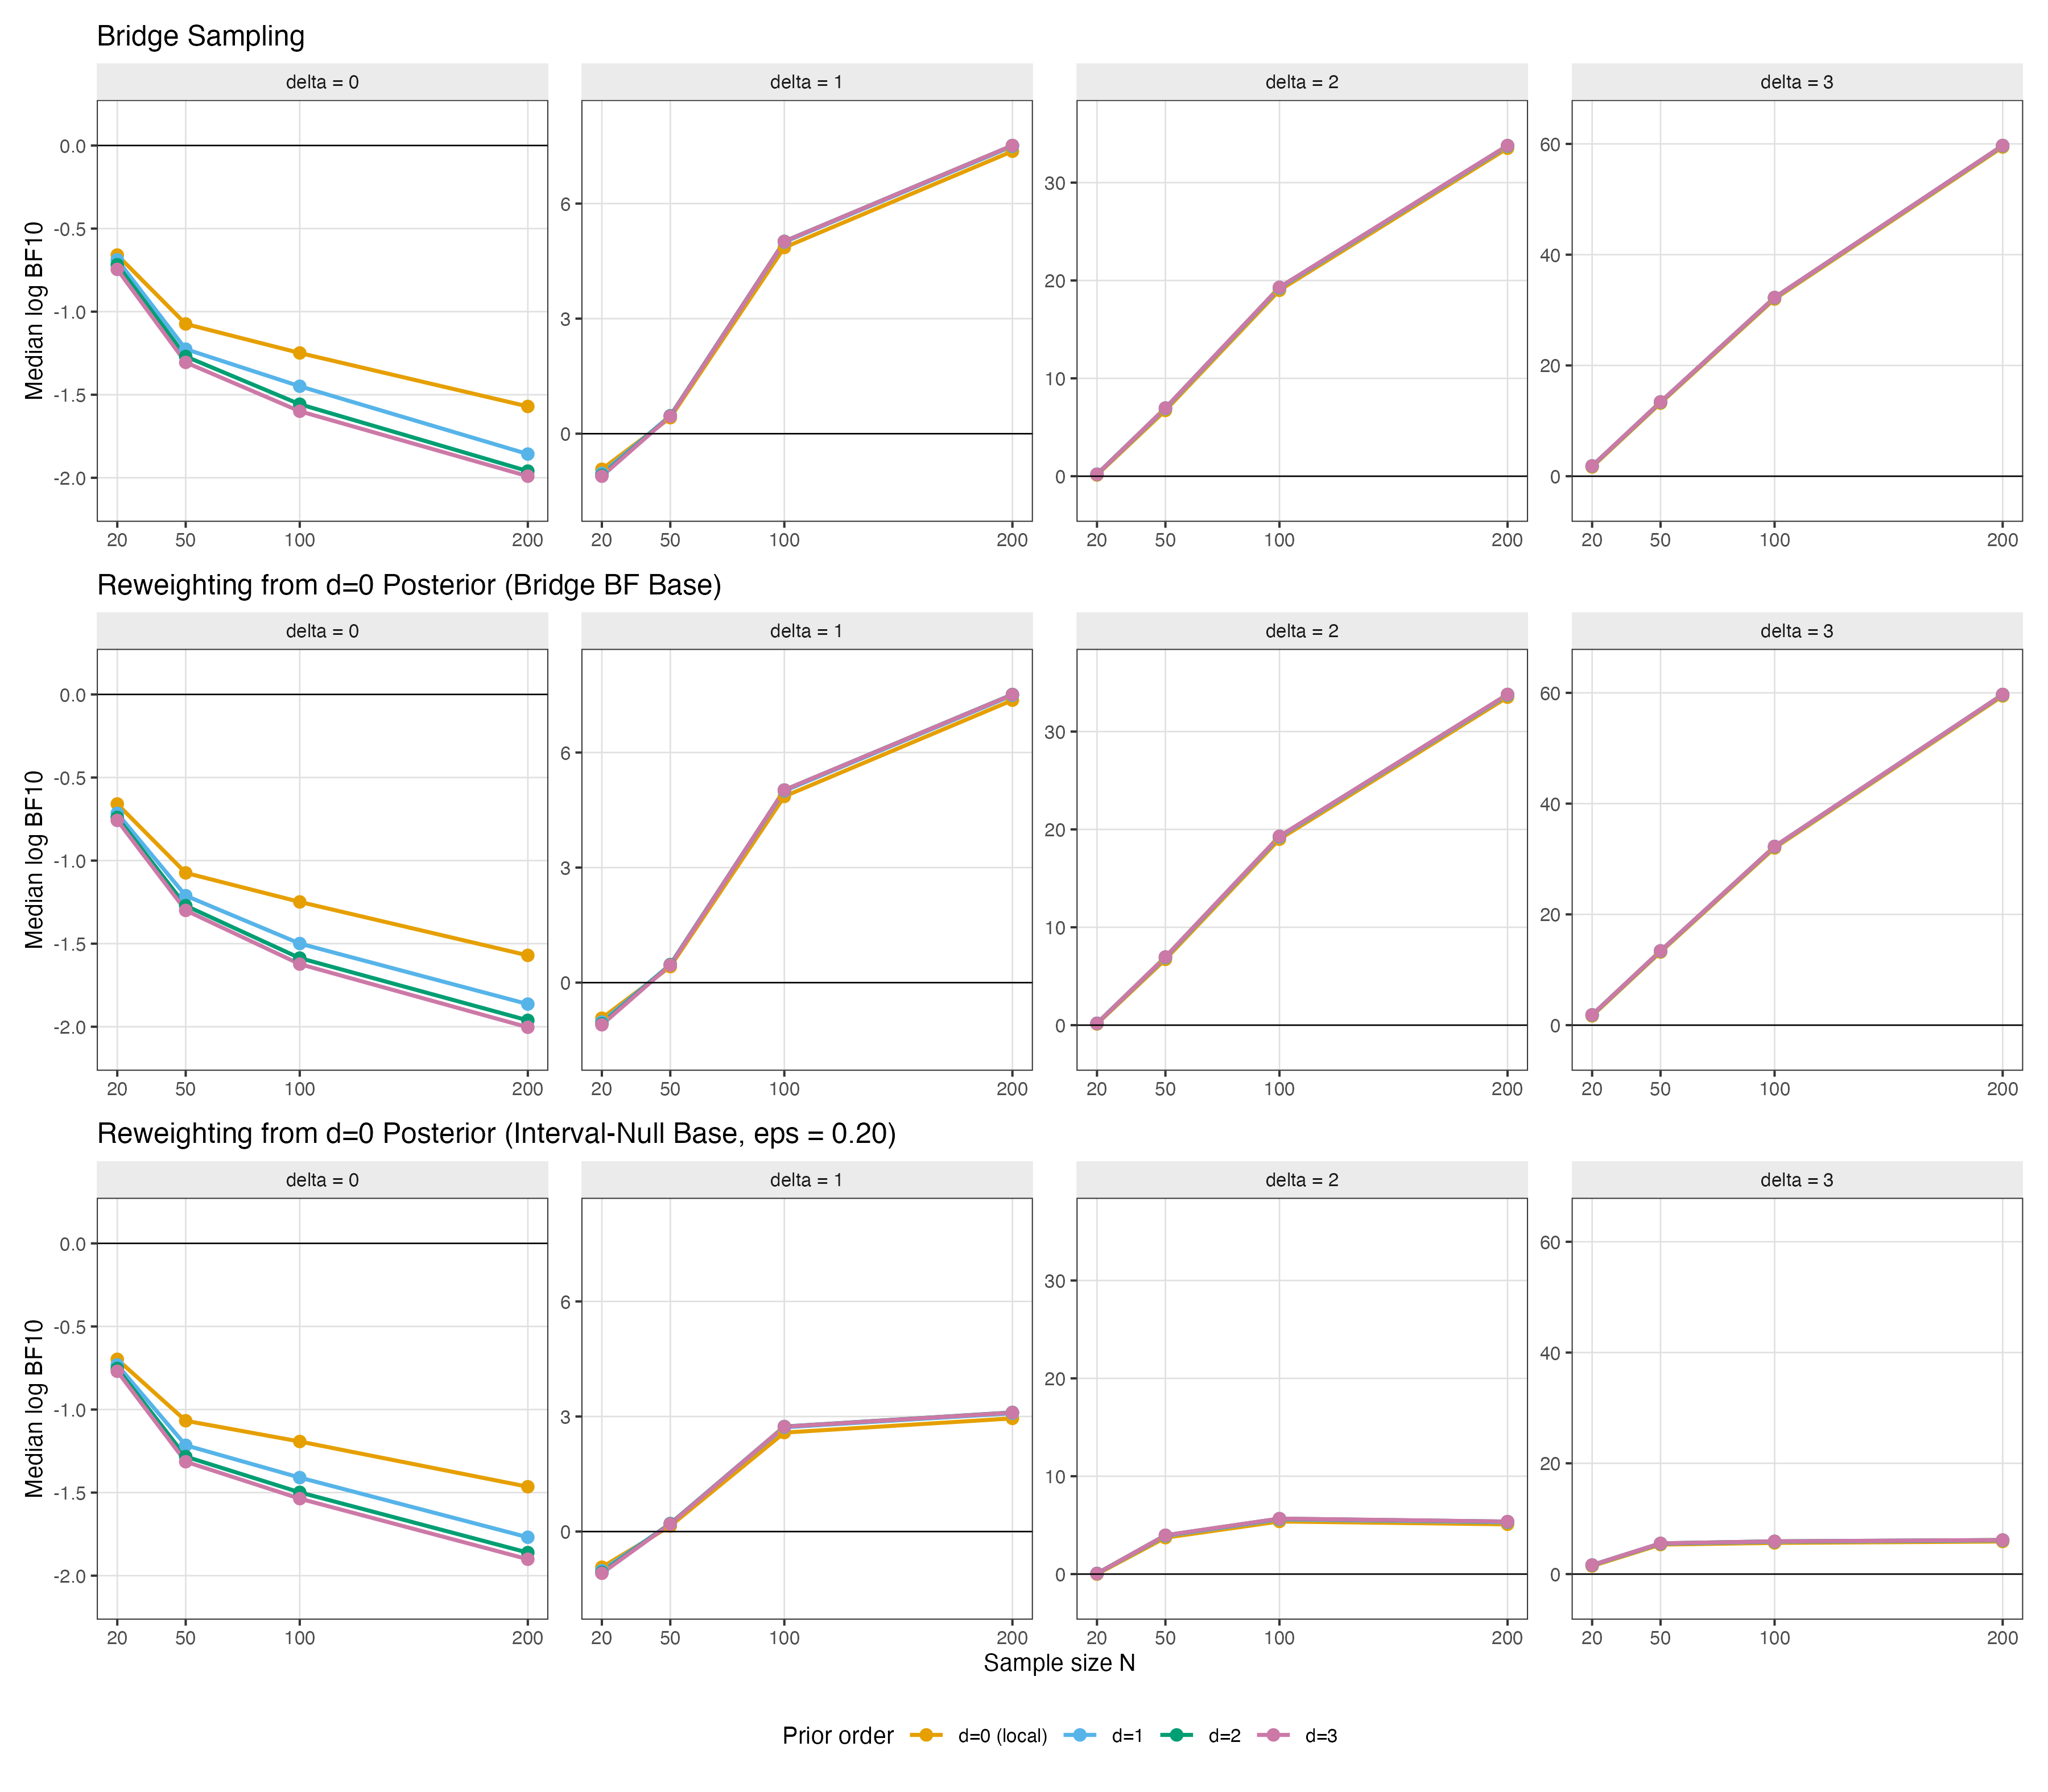
\includegraphics[width=\textwidth]{images/plot-sim-reweighting.png}
  \caption{Simulation results for nonlinear-effect Bayes factors under
  $\delta \in \{0,1,2,3\}$, $N \in \{20,50,100,200\}$, fixed
  $\lambda=0.3$, and prior orders $d \in \{0,1,2,3\}$. Columns
  correspond to the true nonlinear magnitude $\delta$, and colors denote
  the prior order. The first row shows direct bridge-sampling Bayes
  factors. The second row shows Bayes factors obtained by reweighting
  from the $d=0$ posterior using the bridge-sampling Bayes factor as the
  base quantity. The third row shows Bayes factors obtained by
  reweighting from the $d=0$ posterior using the interval-null Bayes
  factor with logspline estimation and $\varepsilon=0.2$ as the base
  quantity. Points and lines show median log Bayes factors across 50
  simulated datasets per configuration; Monte Carlo variation across
  replicates is not displayed. Note that the vertical scale is free
  across columns, reflecting the rapid growth of the Bayes factor with
  $\delta$.}
  \label{fig:simulation-bf}
\end{figure*}

\section{Empirical Application\label{sec:empirical}}
\subsection{Facebook Friends Versus Grey Matter}
\textcite{kanai2012} collected structural MRI data from a sample of $N=40$ university students, quantifying each individual's number of Facebook friends and measuring grey matter volume across brain regions implicated in social cognition and emotional processing—such as the superior temporal sulcus, prefrontal cortex, entorhinal cortex, and amygdala—to examine whether online social network size correlates with brain anatomy. Subsequent reanalysis using traditional null-hypothesis significance testing confirmed a statistically significant positive correlation between the square root of the number of Facebook friends and grey matter density, and \textcite{wetzels2012} further assessed the data using their default Bayesian correlation test, which provided Bayes factor–based support for a nonzero association between social network size and brain structure.

Our method refines this conclusion by separating evidence for a linear association from evidence for a nonlinear departure. The linear effect is tested with the Savage--Dickey ratio and the nonlinear effect with the interval-null Bayes factor ($\varepsilon=0.2$) under the local prior ($d=0$). The log Bayes factor for the linear effect was $\log\mathrm{BF}_{10}=2.36$, indicating positive evidence that Facebook-friend count is associated with grey matter density. In contrast, the interval-null log Bayes factor for the nonlinear effect was $\log\mathrm{BF}_{10}=-1.17$, indicating that the data do not support an additional nonlinear component beyond the linear trend. The reweighted nonlinear log Bayes factors under the non-local priors were also all negative ($\log\mathrm{BF}_{10}=-1.33$, $-1.40$, and $-1.44$ for $d=1,2,3$, respectively), reinforcing the same conclusion. Figure~\ref{fig:neuro_trend} is consistent with this result: the estimated GP trend is nearly indistinguishable from the linear fit across the observed predictor range, with the posterior uncertainty band showing no clear systematic departure from linearity.

\begin{figure}[t]
  \centering
  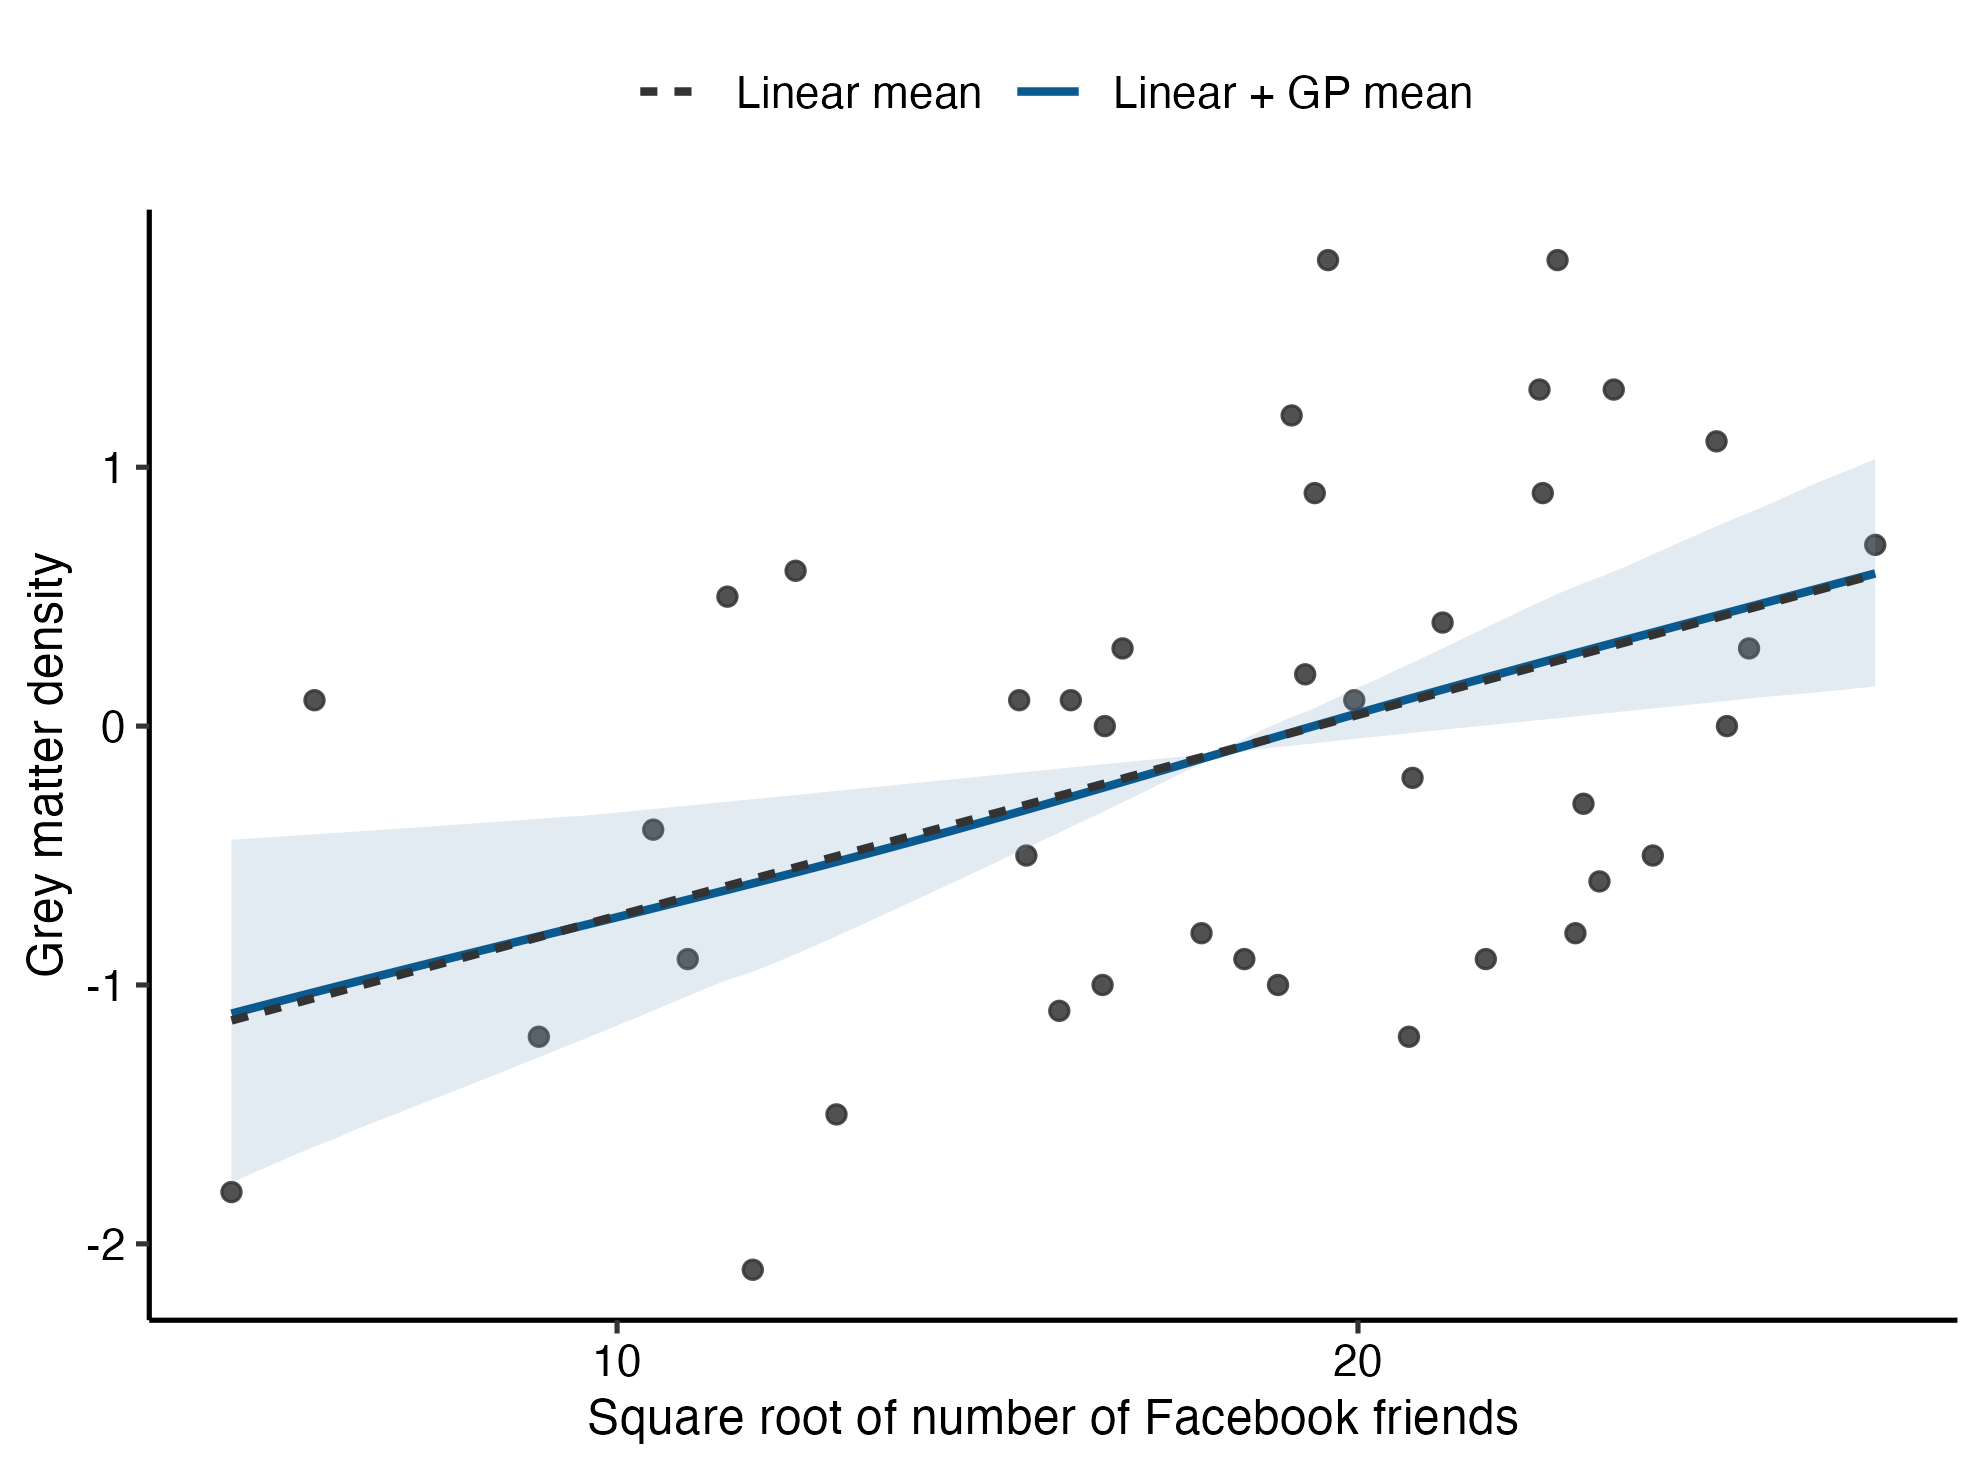
\includegraphics[width=0.82\textwidth]{images/fig_01_neuro_trend.png}
  \caption{Square root of the number of Facebook friends (horizontal) versus grey matter density (vertical). The dashed line shows the posterior mean under the linear component, and the solid line shows the posterior mean under the additive GP model; the shaded region is the 95\% credible band for the full model. The two fitted trends nearly overlap, consistent with the Bayes-factor evidence for a linear association without an additional nonlinear effect.}
  \label{fig:neuro_trend}
\end{figure}


\subsection{Mother's IQ vs.\ Child Test Scores}

We analyze data from a subsample of the National Longitudinal Survey of Youth, focusing on the relationship between mothers' IQ scores and their children's test scores. The dataset, described by \textcite{gelman2007}, contains $n = 434$ mother--child pairs together with a binary indicator of whether the mother completed high school (HS${}=1$: 341 mothers; HS${}=0$: 93 mothers). This application exercises the group-interaction extension of the framework: in addition to testing whether the common trend between mother's IQ and child test scores is nonlinear, we test whether any nonlinear structure in that trend differs between the two education groups.

We use deviation coding for the group indicator, $z_i\in\{-\tfrac{1}{2},+\tfrac{1}{2}\}$ for HS${}=0$ and HS${}=1$ respectively, so that $f_{\text{main}}$ represents the grand-mean nonlinear trend across groups and $f_{\text{int}}$ represents a symmetric group-specific deviation. Writing $x$ for mother's IQ, the model is
%
\begin{equation}
  y_i \;=\; \beta_0 + \beta_1 x_i
         \;+\; f_{\text{main}}(x_i)
         \;+\; z_i\,f_{\text{int}}(x_i)
         \;+\; \varepsilon_i,
  \qquad
  \varepsilon_i\sim\mathcal{N}(0,\sigma^2),
\end{equation}
%
\begin{equation}
  f_{\text{main}}\sim \mathcal{GP}\!\bigl(0,\;
      \sigma^2\delta_{\text{main}}^{\,2}\,
      \widetilde{K}_{\lambda_{\text{main}}}\bigr),
  \qquad
  f_{\text{int}}\sim \mathcal{GP}\!\bigl(0,\;
      \sigma^2\delta_{\text{int}}^{\,2}\,
      \widetilde{K}_{\lambda_{\text{int}}}\bigr),
\end{equation}
%
where both orthogonalized kernels $\widetilde{K}$ are constructed following Section~\ref{subsec:gp}. The linear mean $\beta_0+\beta_1 x_i$ therefore absorbs all linear structure; the Bayes factor for $\delta_{\text{main}}=0$ tests whether a common nonlinear trend is needed beyond the linear effect, and the Bayes factor for $\delta_{\text{int}}=0$ tests whether any nonlinear deviation from that common trend differs between the two groups. The moment prior of order $d=0$ (local prior) is applied to both $\delta_{\text{main}}$ and $\delta_{\text{int}}$.

We report interval-null Bayes factors ($\varepsilon = 0.2$) for the nonlinear main effect ($\delta_{\text{main}}$) and the nonlinear interaction ($\delta_{\text{int}}$), with bridge sampling as an independent benchmark. The interval-null and bridge-sampling estimates are shown in Table~\ref{tab:bf_education}.

\begin{table}[t]
  \centering
  \caption{Log Bayes factors ($\log\mathrm{BF}_{10}$) for nonlinear effects in the mother's IQ model. IN: interval-null Bayes factor ($\varepsilon = 0.2$, local prior $d=0$); BS: bridge sampling.}
  \label{tab:bf_education}
  \begin{tabular}{lcc}
    \toprule
    Component & $\log\mathrm{BF}_{10}^{\text{IN}}$ & $\log\mathrm{BF}_{10}^{\text{BS}}$ \\
    \midrule
    Main (nonlinear)        & 2.09   & 3.60  \\
    Interaction (nonlinear) & -0.53  & -0.56  \\
    \bottomrule
  \end{tabular}
\end{table}

There is strong evidence for a common nonlinear relationship between mother's IQ and child test scores. For the nonlinear interaction, both methods agree closely and yield log Bayes factors below~zero, indicating no evidence that the nonlinear trend differs between mothers who did and did not complete high school.

Figure~\ref{fig:education} displays the estimated trends. The common nonlinear trend (dashed) shows a clear departure from linearity, with a steeper rise in child test scores at lower maternal IQ values that flattens toward the upper range. The group-specific curves (solid) nearly overlap with the common trend, consistent with the weak interaction Bayes factor. Together, the results indicate that the association between mother's IQ and child test scores is well characterized by a shared nonlinear trend that does not differ appreciably between the two education groups.

\begin{figure}[t]
  \centering
  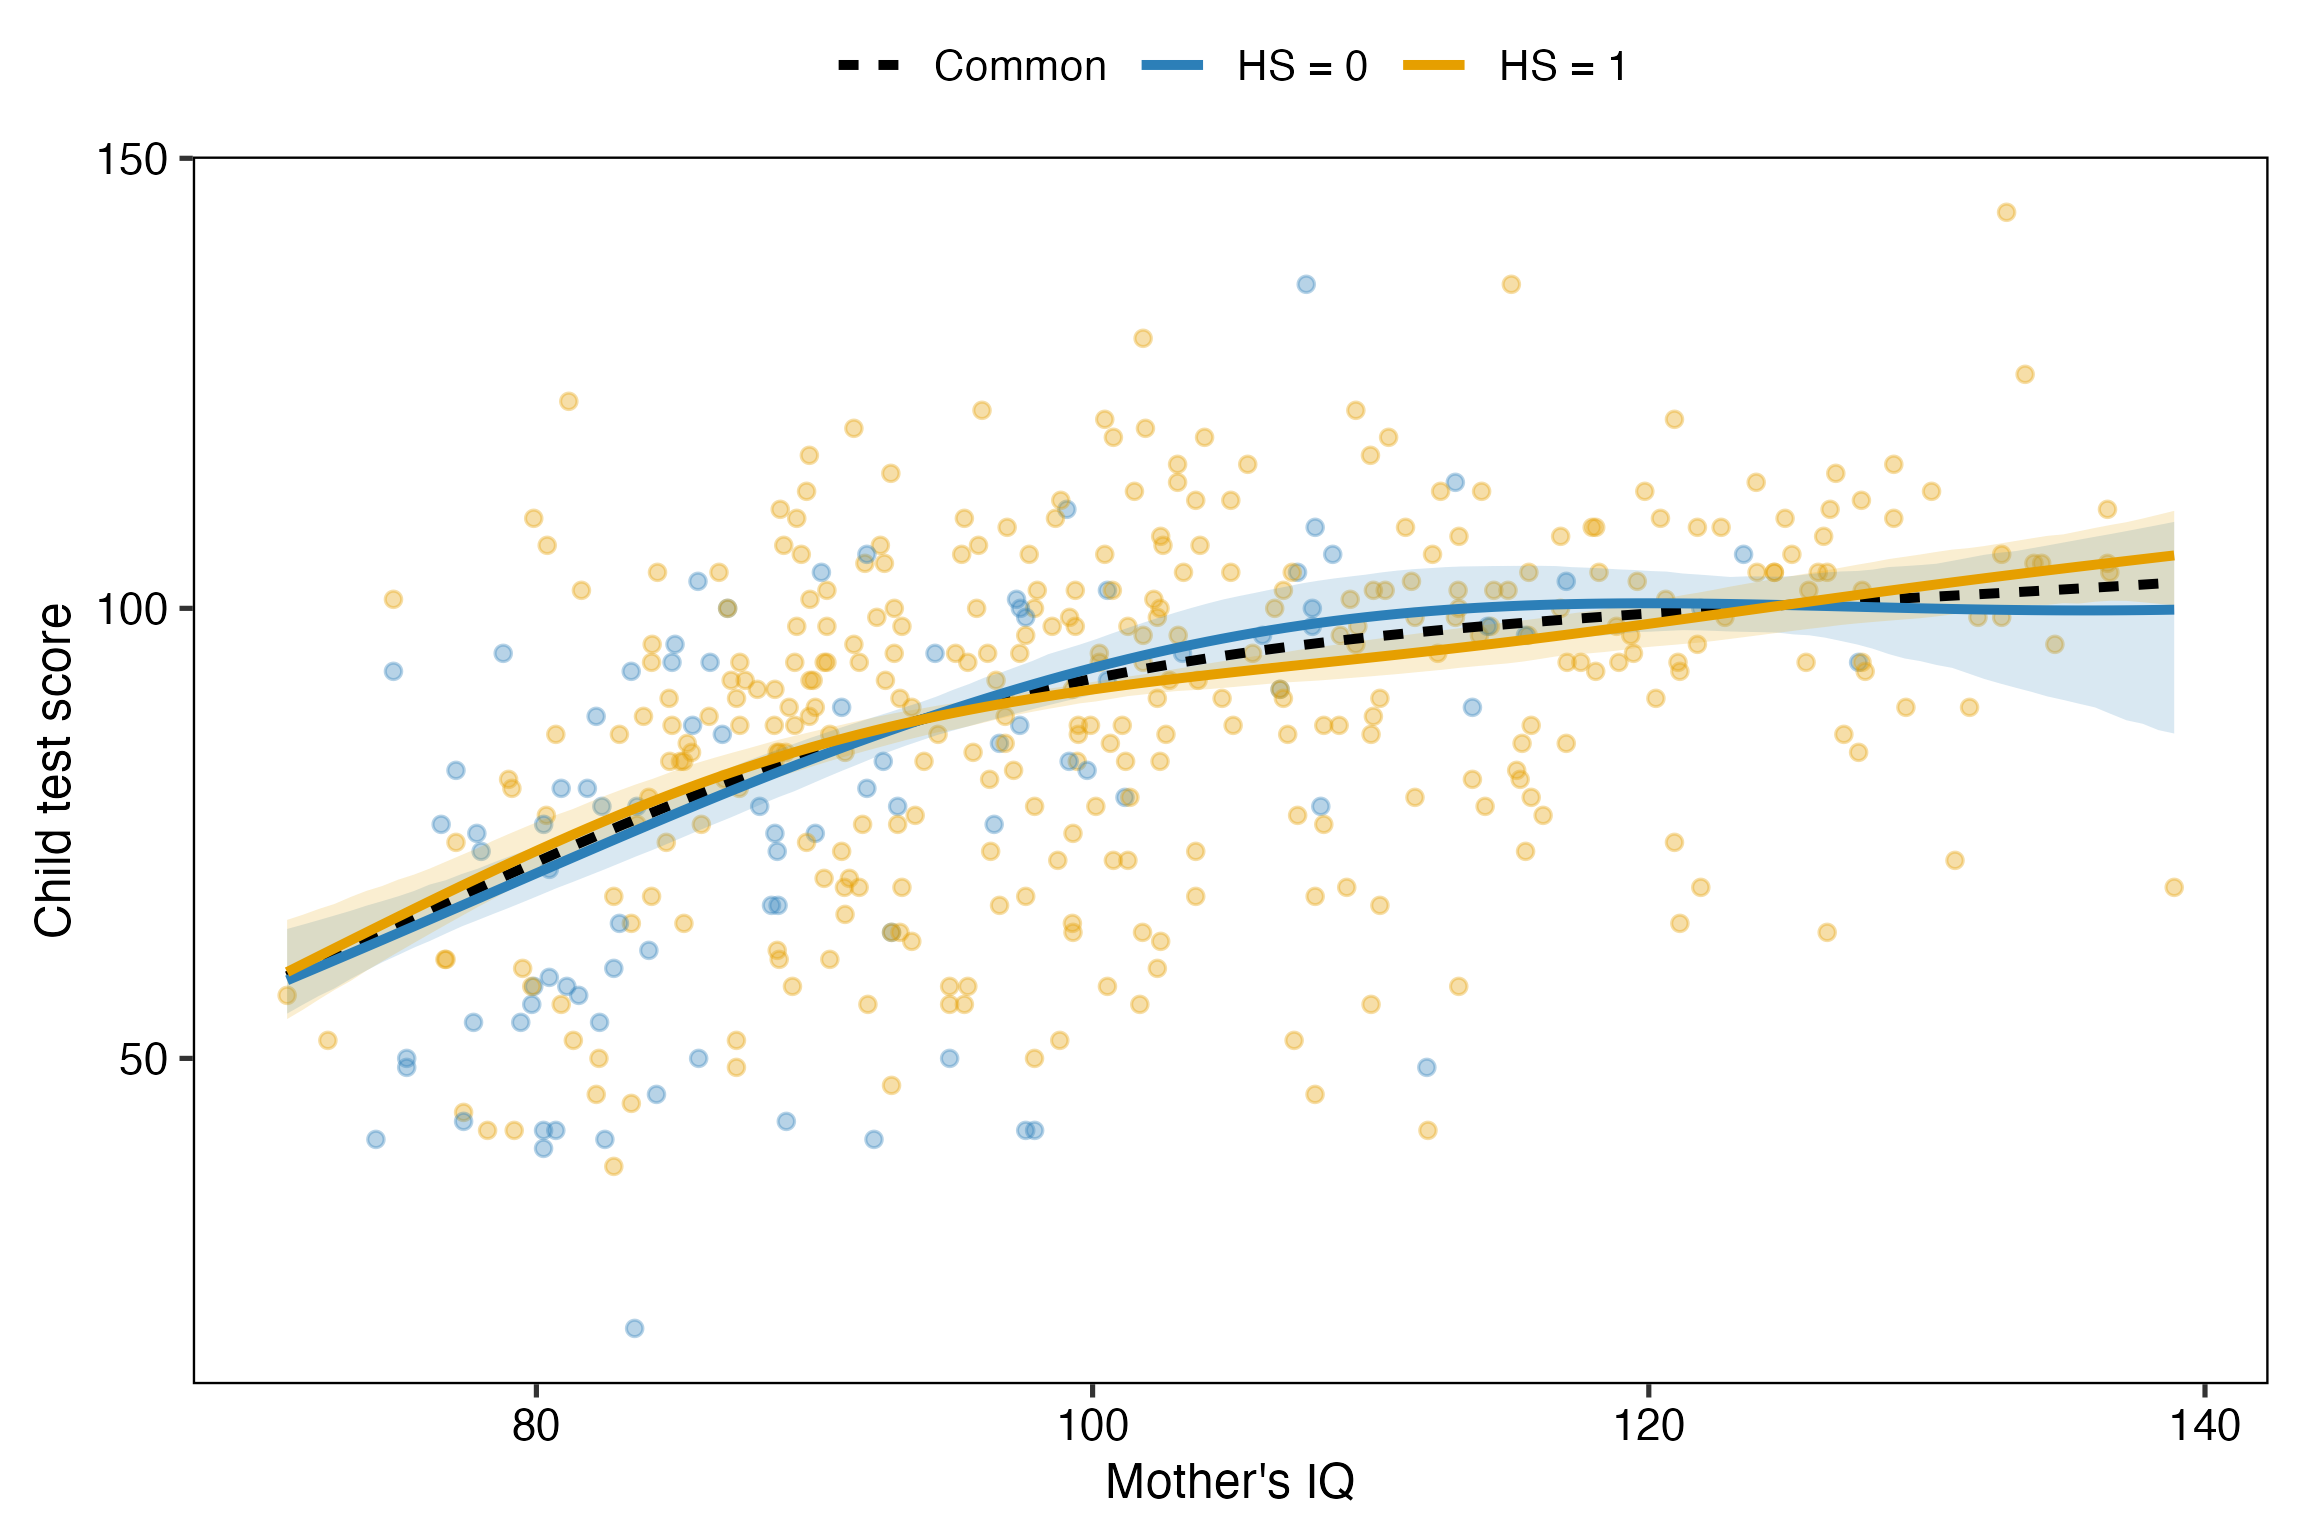
\includegraphics[width=\textwidth]{images/fig_education_trends.png}
  \caption{Mother's IQ (horizontal) vs.\ child test scores (vertical). The dashed black curve shows the estimated common nonlinear trend; solid curves show group-specific trends (blue for HS${}\,=\,0$, orange for HS${}\,=\,1$), with shaded regions indicating $95\%$ credible intervals. Points show the observed data for each group.}
  \label{fig:education}
\end{figure}

\subsection{Diabetes Dataset}

The diabetes dataset of \textcite{efron2004} records disease progression for $n=442$ patients. Setting aside the binary variable \texttt{sex}, we fit the additive GP model to the nine continuous baseline predictors: \texttt{age}, \texttt{bmi}, \texttt{bp} (mean arterial pressure), and six blood serum measurements, corresponding to total cholesterol (\texttt{s1}), LDL (\texttt{s2}), HDL (\texttt{s3}), total cholesterol/HDL (\texttt{s4}), log triglycerides (\texttt{s5}), and glucose (\texttt{s6}).\footnote{This naming convention is standard for the diabetes benchmark dataset.} In benchmark analyses, \textcite{efron2004} used this dataset to illustrate the LARS/LASSO solution paths, and \textcite{park2008bayesian} applied the Bayesian Lasso; both studies highlight that only a small subset of predictors carries most of the predictive signal, with \texttt{bmi}, \texttt{bp}, and \texttt{s5} repeatedly among the most important. This earlier literature provides a useful benchmark for our decomposition, because it identifies influential predictors but does not distinguish whether their contribution is primarily linear or nonlinear.

\begin{table}[t]
  \centering
  \caption{Predictor-specific evidence in the Diabetes dataset. The Bayes-factor columns report $\log(\mathrm{BF}_{10})$ for the linear and nonlinear effects, computed with the Savage--Dickey ratio for the linear effect and the interval-null Bayes factor ($\varepsilon=0.2$, local prior $d=0$) for the nonlinear effect. The ARD column reports the inverse range from the anisotropic GP baseline, so larger values indicate shorter length-scales and greater overall GP sensitivity.}
  \label{tab:diabetes_bf_ard}
  \small
  \begin{tabular}{lrrr}
    \toprule
    Predictor & Linear & Nonlinear & ARD \\
    \midrule
    age & -2.87 & -0.74 & 0.139 \\
    bmi & 16.31 & -1.24 & 0.173 \\
    bp  & 4.77  & -1.71 & 0.107 \\
    s1  & -1.52 & -1.68 & 0.050 \\
    s2  & -2.24 & -1.11 & 0.000 \\
    s3  & -2.78 & -1.57 & 0.055 \\
    s4  & -2.67 & -1.67 & 0.000 \\
    s5  & 5.57  & -0.60 & 0.262 \\
    s6  & -2.73 & -0.61 & 0.083 \\
    \bottomrule
  \end{tabular}
\end{table}

Table~\ref{tab:diabetes_bf_ard} shows that the diabetes signal is predominantly linear. The strongest evidence for linear effects is concentrated on \texttt{bmi}, \texttt{s5}, and \texttt{bp}, whereas the remaining predictors have negative log Bayes factors for the linear component. This agrees closely with the classical importance pattern reported by \textcite{efron2004} and \textcite{park2008bayesian}, and sharpens it by showing that the support for these predictors is carried mainly through linear effects rather than through nonlinear departures. For the nonlinear component, all predictors have negative log Bayes factors. Within the present additive GP decomposition, we find little evidence that these predictor effects arise from pronounced nonlinear structure. The full marginal posteriors of the linear and nonlinear parameters for this application are shown in Appendix~\ref{app:posteriors} (Figures~\ref{fig:post-a3-theta} and~\ref{fig:post-a3-delta}).

The ARD comparison is qualitatively consistent with this interpretation, but it is less specific. Predictors such as \texttt{s5}, \texttt{bmi}, and \texttt{bp} receive relatively short ARD ranges, which agrees with their overall importance, yet ARD does not reveal that this importance is primarily linear. The contrast is most visible for \texttt{age} and \texttt{s6}: both receive moderate ARD scores despite weak evidence for either a linear or a nonlinear effect in our decomposition. At the other extreme, \texttt{s2} and \texttt{s4} receive ARD ranges of essentially zero, indicating that the anisotropic GP effectively switches these predictors off. This illustrates the role of ARD in our study: it provides a coarse GP-based sensitivity summary, whereas the proposed Bayes-factor analysis separates evidence for linear and nonlinear contributions.

\subsection{Boston Housing Dataset}

The Boston Housing dataset, originally compiled by \textcite{harrison1978}, contains data on 506 census tracts in the Boston area and has become a standard benchmark for regression and variable selection methods. In our analysis, we exclude the binary predictor \texttt{chas} and the ordinal accessibility measure \texttt{rad}, and retain the 11 continuous predictors \texttt{crim}, \texttt{zn}, \texttt{indus}, \texttt{nox}, \texttt{rm}, \texttt{age}, \texttt{dis}, \texttt{tax}, \texttt{ptratio}, \texttt{black}, and \texttt{lstat}.\footnote{The \texttt{black} predictor is a transformed measure of racial composition, $1000(\mathrm{Bk}-0.63)^2$, whose construction and ethical implications have been widely criticized; it has since been removed from several standard distributions of the dataset. We retain it here only for comparability with earlier analyses and draw no substantive conclusions from it.} The response variable is the median value of owner-occupied homes (in thousands of dollars). This dataset has been analyzed repeatedly as a variable-selection benchmark, and GP-based analyses in particular often emphasize predictors such as \texttt{nox}, \texttt{rm}, \texttt{dis}, \texttt{tax}, and \texttt{lstat}. In a directly relevant comparison, \textcite{savitsky2011} used a fully multivariate GP with spike-and-slab selection on kernel parameters and also highlighted these variables as important. These earlier findings provide a natural reference point for our results.

\begin{table}[t]
  \centering
  \caption{Predictor-specific evidence in the Boston Housing dataset. The Bayes-factor columns report $\log(\mathrm{BF}_{10})$ for the linear and nonlinear effects, computed with the Savage--Dickey ratio for the linear effect and the interval-null Bayes factor ($\varepsilon=0.2$, local prior $d=0$) for the nonlinear effect. The ARD column reports the inverse range from the anisotropic GP baseline, so larger values indicate shorter length-scales and greater overall GP sensitivity.}
  \label{tab:boston_bf_ard}
  \small
  \begin{tabular}{lrrr}
    \toprule
    Predictor & Linear & Nonlinear & ARD \\
    \midrule
    crim    & 2.14  & 1.34  & 0.093 \\
    zn      & 5.35  & -1.51 & 0.003 \\
    indus   & -2.49 & 0.98  & 0.133 \\
    nox     & 8.49  & 5.69  & 0.450 \\
    rm      & 32.36 & 6.52  & 0.243 \\
    age     & -3.05 & -1.91 & 0.172 \\
    dis     & 25.56 & 5.86  & 0.792 \\
    tax     & -2.94 & 3.89  & 1.054 \\
    ptratio & 20.59 & -1.46 & 0.098 \\
    black   & 5.97  & -0.87 & 0.312 \\
    lstat   & 27.53 & 4.15  & 0.566 \\
    \bottomrule
  \end{tabular}
\end{table}

Table~\ref{tab:boston_bf_ard} shows a substantially richer pattern than in the diabetes application. Several predictors display strong linear evidence, especially \texttt{rm}, \texttt{lstat}, \texttt{dis}, \texttt{ptratio}, and \texttt{nox}, with additional positive support for \texttt{black}, \texttt{zn}, and \texttt{crim}. At the same time, the nonlinear analysis identifies clear departures from linearity for \texttt{nox}, \texttt{rm}, \texttt{dis}, \texttt{tax}, and \texttt{lstat}, while \texttt{crim} and \texttt{indus} show weaker but still positive nonlinear support. This is broadly consistent with previous work, especially the emphasis on \texttt{nox}, \texttt{rm}, \texttt{dis}, \texttt{tax}, and \texttt{lstat}, but the present decomposition is more informative. In particular, it suggests that \texttt{tax} is supported mainly through a nonlinear component, whereas \texttt{ptratio}, \texttt{zn}, and \texttt{black} are supported mainly through linear effects. The corresponding marginal posteriors are reported in Appendix~\ref{app:posteriors} (Figures~\ref{fig:post-a4-theta} and~\ref{fig:post-a4-delta}).

The ARD results show clearer qualitative agreement with our nonlinear findings here than in the diabetes application. Predictors with strong nonlinear evidence under our method—especially \texttt{tax}, \texttt{dis}, \texttt{lstat}, \texttt{nox}, and \texttt{rm}—also tend to have relatively short ARD ranges. The agreement is nevertheless not exact. The variable \texttt{black} is a useful counterexample: it receives a comparatively large ARD score, yet our analysis yields weak nonlinear evidence and stronger support for a linear effect. This again underscores the distinction between the two approaches. ARD summarizes overall sensitivity of the fitted GP surface, whereas the proposed Bayes-factor analysis separates that sensitivity into evidence for linear and nonlinear structure.

\section{Discussion\label{sec:discussion}}

We have proposed a Bayesian framework for weighing the evidence for
linear and nonlinear effects in additive Gaussian process regression.
The starting point is an orthogonalized GP construction that separates
each predictor's linear trend from its nonlinear departure. This
separation lets a single standardized magnitude parameter~$\delta_j$
summarize the strength of the nonlinear component, so that testing for
nonlinearity reduces to a scalar point-null hypothesis. Because all of
the resulting Bayes factors are computed from one fit of the full model,
through the Savage--Dickey density ratio and its encompassing-prior
extension, no separate null and alternative models need be estimated.
Placing non-local priors on $\delta_j$ then sharpens the contrast
between the competing hypotheses, while the interval-null Bayes factor
remains well defined in the regime where the pointwise Savage--Dickey
ratio does not, and bridge sampling provides an independent benchmark.

These properties held up in practice. The simulation study confirmed
that the bridge-sampling Bayes factor behaves as a benchmark should,
growing with both the nonlinear signal and the sample size, and that
the reweighting identity reproduces the non-local-prior Bayes factors
almost exactly, so that an entire family of prior orders can be read off
a single fit. The interval-null Bayes factor was accurate near the null
and became conservative once the posterior moved well beyond it, yet it
never reversed the direction of the evidence and consistently
distinguished negligible from substantial nonlinear effects---the
behavior one wants from a screening tool, even where it understates the
strength of a pronounced effect.

The applications show what this resolution buys in interpretation. In
every case the decomposition reported not merely whether a predictor
mattered but how it mattered---linearly, nonlinearly, or not at
all---a distinction that global relevance measures such as ARD cannot
draw. Facebook friendships were related to grey matter density through a
purely linear trend, and mother's IQ to child test scores through a
nonlinear main effect that did not vary with maternal education. The
diabetes data placed most of their support on a handful of largely
linear predictors, whereas the Boston Housing data combined strong
linear effects with clearly nonlinear ones.

Several limitations and extensions deserve comment. The framework relies
on exact GP inference and therefore scales as $\mathcal{O}(n^3)$ per
iteration, which becomes burdensome when Bayes factors are needed across
many specifications or when $n$ grows beyond a few hundred. We used
exact inference to isolate the behavior of the Bayes factor machinery
from approximation error; integrating sparse pseudo-input methods
\parencite{snelson2006sparse, quinoneroCandela2005unifying},
variational inducing-point schemes \parencite{titsias2009variational,
hensman2013gaussian}, or Hilbert space approximations
\parencite{riutortMayol2023hsgp} would improve scalability, but whether
these approximations preserve the theoretical guarantees of the
interval-null Bayes factor (Appendix~\ref{app:interval-limit}) is a
non-trivial question that we leave for future work. A further caveat
concerns the simulation design: the true length-scale there was fixed at
the prior median, so the reported behavior does not speak to robustness
under length-scale misspecification, which a dedicated sensitivity study
could address.

A more substantive extension concerns model structure. The present
framework treats nonlinear contributions additively, with one component
per predictor. Replacing each univariate component $f_j(x_j)$ with a
component $f_S(\mathbf{x}_S)$ indexed by a subset
$S \subseteq \{1,\dots,p\}$ yields a functional ANOVA-style decomposition
in which each component carries its own standardized magnitude~$\delta_S$
and its own orthogonalized kernel, with higher-order components
orthogonalized against lower-order ones to retain identifiability. The same Bayes factor
machinery would then test whether a specific interaction structure is
supported by the data, moving the framework from marginal variable
importance toward direct evidence for interaction structure. The
practical difficulty is combinatorial: exhaustive search over $2^p$
subsets is infeasible beyond small~$p$, so a usable version would
restrict attention to low-order interactions or employ hierarchical
search in the spirit of \textcite{duvenaud2013structure}.

The framework is also not tied to a particular covariance kernel. We
used the squared-exponential kernel for concreteness, but the infinite
differentiability of its sample paths imposes more smoothness than many
applied settings warrant \parencite{stein1999interpolation}. The Mat\'ern
family provides a standard alternative that indexes sample-path
regularity through a parameter~$\nu > 0$:
\begin{equation}
k_{\nu}(x, x' \mid \lambda_j)
  = \frac{2^{1-\nu}}{\Gamma(\nu)}
    \!\left(\frac{\sqrt{2\nu}\,|x-x'|}{\lambda_j}\right)^{\!\nu}
    K_{\nu}\!\left(\frac{\sqrt{2\nu}\,|x-x'|}{\lambda_j}\right),
\end{equation}
where $K_{\nu}$ is the modified Bessel function of the second kind;
common choices are $\nu=3/2$ and $\nu=5/2$, with $\nu\to\infty$
recovering the squared-exponential kernel. Because the standardized
parameterization normalizes the kernel so that $k(x,x)=1$, the
nonlinear component in~\eqref{eq:prior-fj} remains
$\sigma^2\delta_j^{\,2}\widetilde{\mathbf{K}}_j$ regardless of the
kernel choice, the orthogonalization in~\eqref{eq:ortho-kernel} applies
verbatim, and $\delta_j$ retains its signal-to-noise interpretation.
The Bayes factor machinery thus transfers without modification, and
systematic comparison of kernels is a natural follow-up.

Finally, with $p$ predictors the framework produces $2p$ Bayes factors
per model fit (22 for the Boston Housing application), and reporting
these without accounting for multiplicity can inflate the joint rate of
false discoveries. A principled Bayesian response is to place a prior on
the joint inclusion pattern of the linear and nonlinear components,
which automatically imposes multiplicity adjustment through the
resulting shrinkage on inclusion probabilities
\parencite{scott2010}; incorporating such a prior into the present
framework, together with decision rules calibrated to a joint error
criterion, would strengthen the procedure in higher-dimensional
applications.

Taken together, these extensions would broaden the reach of the
framework, but its core contribution---separating linear from nonlinear
evidence within a single coherent Bayes-factor analysis---already
applies directly to the additive models common in applied practice.

\appendix

\section{Limit of the interval-null Bayes factor}
\label{app:interval-limit}
 
We show that
$\lim_{\varepsilon\to 0}
  \mathrm{BF}_{10}^{(\varepsilon)} = \mathrm{BF}_{10}$
for the moment prior $\pi_d(\delta)=\delta^d\,g(\delta)/C_d$
of order $d\ge 0$.
 
Write $N(\varepsilon)$ and $D(\varepsilon)$ for the numerator and
denominator of~\eqref{eq:bf-interval}:
\[
N(\varepsilon) = \int_0^{\varepsilon}\pi_d(\delta)\,d\delta,
\qquad
D(\varepsilon) = \int_0^{\varepsilon}\pi_d(\delta\mid\mathbf{y})
  \,d\delta.
\]
Both are continuous, vanish at $\varepsilon=0$, and are
differentiable for $\varepsilon>0$ by the fundamental theorem of
calculus, with
\[
N'(\varepsilon) = \pi_d(\varepsilon), \qquad
D'(\varepsilon) = \pi_d(\varepsilon\mid\mathbf{y}).
\]
 
\paragraph{Case $d=0$ (local prior).}
Here $\pi_0(0)=g(0)/C_0>0$ and, by assumption, the conditional
marginal likelihood $p(\mathbf{y}\mid\delta)$ is continuous and
positive at $\delta=0$, so
$\pi_0(0\mid\mathbf{y})>0$.
Since $N(0)=D(0)=0$ and $D'(0)=\pi_0(0\mid\mathbf{y})>0$,
l'H\^opital's rule gives
\[
\lim_{\varepsilon\to 0}
  \frac{N(\varepsilon)}{D(\varepsilon)}
= \frac{N'(0)}{D'(0)}
= \frac{\pi_0(0)}{\pi_0(0\mid\mathbf{y})},
\]
which is the Savage--Dickey density ratio and equals
$\mathrm{BF}_{10}$ by the identity of
\textcite{Dickey1971, verdinelli1995}.
 
\paragraph{Case $d\ge 1$ (non-local prior).}
Both $\pi_d(\delta)$ and $\pi_d(\delta\mid\mathbf{y})$ vanish at
$\delta=0$, so a single application of l'H\^opital's rule yields
$0/0$ again.
We proceed by characterizing the local behavior of both densities
near the origin.
 
Because $g$ is continuous with $g(0)>0$, the prior satisfies
\begin{equation}
\label{eq:prior-local-behavior}
\pi_d(\delta) = \frac{\delta^d\,g(\delta)}{C_d}
  \;\sim\; \frac{g(0)}{C_d}\,\delta^d
  \qquad\text{as } \delta\to 0.
\end{equation}
For the posterior, Bayes' theorem gives
\[
\pi_d(\delta\mid\mathbf{y})
  = \frac{p(\mathbf{y}\mid\delta)\,\pi_d(\delta)}
         {p(\mathbf{y}\mid M_1)},
\]
where $p(\mathbf{y}\mid\delta)
  = \int p(\mathbf{y}\mid\delta,\boldsymbol{\eta})\,
    \pi(\boldsymbol{\eta})\,d\boldsymbol{\eta}$
is the conditional marginal likelihood, integrating over the
nuisance parameters $\boldsymbol{\eta}=(\boldsymbol{\theta},
\boldsymbol{\lambda},\sigma^2)$.
By assumption, $p(\mathbf{y}\mid\delta)$ is continuous and positive
at $\delta=0$; in particular,
$p(\mathbf{y}\mid\delta=0)=p(\mathbf{y}\mid M_0)>0$.
Hence
\begin{equation}
\label{eq:post-local-behavior}
\pi_d(\delta\mid\mathbf{y})
  \;\sim\; \frac{p(\mathbf{y}\mid M_0)}{p(\mathbf{y}\mid M_1)}
    \cdot \frac{g(0)}{C_d}\,\delta^d
  \qquad\text{as } \delta\to 0.
\end{equation}
Both densities vanish as $\delta^d$, so their integrals over
$(0,\varepsilon)$ vanish as $\varepsilon^{d+1}$:
\[
N(\varepsilon) \;\sim\; \frac{g(0)}{C_d(d+1)}\,\varepsilon^{d+1},
\qquad
D(\varepsilon) \;\sim\;
  \frac{p(\mathbf{y}\mid M_0)}{p(\mathbf{y}\mid M_1)}
  \cdot \frac{g(0)}{C_d(d+1)}\,\varepsilon^{d+1}.
\]
The numerator and denominator vanish at the same rate, so the
ratio converges to a finite, positive limit
\parencite[cf.][Section~2]{wetzels2010encompassing}:
\begin{equation}
\label{eq:interval-limit-proof}
\lim_{\varepsilon\to 0}
  \frac{N(\varepsilon)}{D(\varepsilon)}
= \frac{g(0)/\bigl[C_d(d+1)\bigr]}
       {\dfrac{p(\mathbf{y}\mid M_0)}{p(\mathbf{y}\mid M_1)}
         \cdot \dfrac{g(0)}{C_d(d+1)}}
= \frac{p(\mathbf{y}\mid M_1)}{p(\mathbf{y}\mid M_0)}
= \mathrm{BF}_{10}.
\end{equation}
All factors involving $g(0)$, $C_d$, and $(d+1)$ cancel,
confirming that the interval Bayes factor recovers the exact
point-null Bayes factor for any prior order $d\ge 0$.
 
Equivalently, applying l'H\^opital's rule $d+1$ times and
using~\eqref{eq:prior-local-behavior}
and~\eqref{eq:post-local-behavior} yields
\[
\lim_{\varepsilon\to 0}
  \frac{N(\varepsilon)}{D(\varepsilon)}
= \lim_{\varepsilon\to 0}
  \frac{N^{(d+1)}(\varepsilon)}{D^{(d+1)}(\varepsilon)}
= \lim_{\varepsilon\to 0}
  \frac{\pi_d^{(d)}(\varepsilon)}
       {\pi_d^{(d)}(\varepsilon\mid\mathbf{y})}
= \frac{d!\,g(0)/C_d}
       {d!\,g(0)\,p(\mathbf{y}\mid M_0)/
         \bigl[C_d\,p(\mathbf{y}\mid M_1)\bigr]}
= \mathrm{BF}_{10},
\]
which confirms the result via the derivative route.
\hfill$\square$


\section{Simulation Bayes factors}
\label{app:sim-table}

\begin{table}[ht]
  \centering
  \caption{Median bridge-sampling log Bayes factors
  ($\log \mathrm{BF}_{10}$) across 50 simulated datasets, by true
  nonlinear magnitude $\delta$, sample size $N$, and prior order
  $d$. Higher prior orders sharpen the evidence in the direction
  favored by the data---more negative when $\delta=0$, more positive
  when $\delta>0$---and the separation across prior orders persists at
  every $\delta$, although it is visually obscured in
  Figure~\ref{fig:simulation-bf} by the expanding vertical scale.}
  \label{tab:bridge-medians}
  \begin{tabular}{ccrrrr}
    \toprule
    & & \multicolumn{4}{c}{Prior order $d$} \\
    \cmidrule(lr){3-6}
    $\delta$ & $N$ & $d=0$ & $d=1$ & $d=2$ & $d=3$ \\
    \midrule
    0 & 20 & -0.66 & -0.69 & -0.72 & -0.75 \\
     & 50 & -1.07 & -1.23 & -1.27 & -1.31 \\
     & 100 & -1.25 & -1.45 & -1.56 & -1.60 \\
     & 200 & -1.57 & -1.86 & -1.96 & -1.99 \\
    \midrule
    1 & 20 & -0.93 & -1.04 & -1.09 & -1.11 \\
     & 50 & 0.42 & 0.47 & 0.47 & 0.46 \\
     & 100 & 4.85 & 5.00 & 5.01 & 5.01 \\
     & 200 & 7.36 & 7.49 & 7.51 & 7.51 \\
    \midrule
    2 & 20 & 0.12 & 0.19 & 0.20 & 0.19 \\
     & 50 & 6.72 & 6.91 & 6.96 & 6.97 \\
     & 100 & 19.00 & 19.20 & 19.30 & 19.30 \\
     & 200 & 33.50 & 33.70 & 33.80 & 33.80 \\
    \midrule
    3 & 20 & 1.67 & 1.82 & 1.86 & 1.86 \\
     & 50 & 13.20 & 13.40 & 13.40 & 13.40 \\
     & 100 & 32.00 & 32.20 & 32.30 & 32.30 \\
     & 200 & 59.40 & 59.60 & 59.70 & 59.70 \\
    \bottomrule
  \end{tabular}
\end{table}

\section{Posterior samples for the diabetes and Boston housing applications}
\label{app:posteriors}

For the two higher-dimensional applications of
Section~\ref{sec:empirical}---the diabetes and Boston housing
datasets---we report the full marginal posterior distributions that
underlie the Bayes factors summarized in the main text. For every
predictor we show the posterior of the nonlinear magnitude $\delta_j$
and of the linear coefficient $\theta_j$ under the additive Gaussian
process model. In each panel the grey histogram is the posterior
sample and the red curve is the corresponding prior density; in the
$\theta_j$ panels the dashed vertical line marks the null value
$\theta_j = 0$. Comparing the posterior with the prior gives a visual
counterpart to the formal Bayes factors: mass of the $\delta_j$
posterior near zero relative to the prior indicates little support for
a nonlinear effect, while concentration of the $\theta_j$ posterior
away from zero indicates a linear effect.

\begin{figure}[ht]
  \centering
  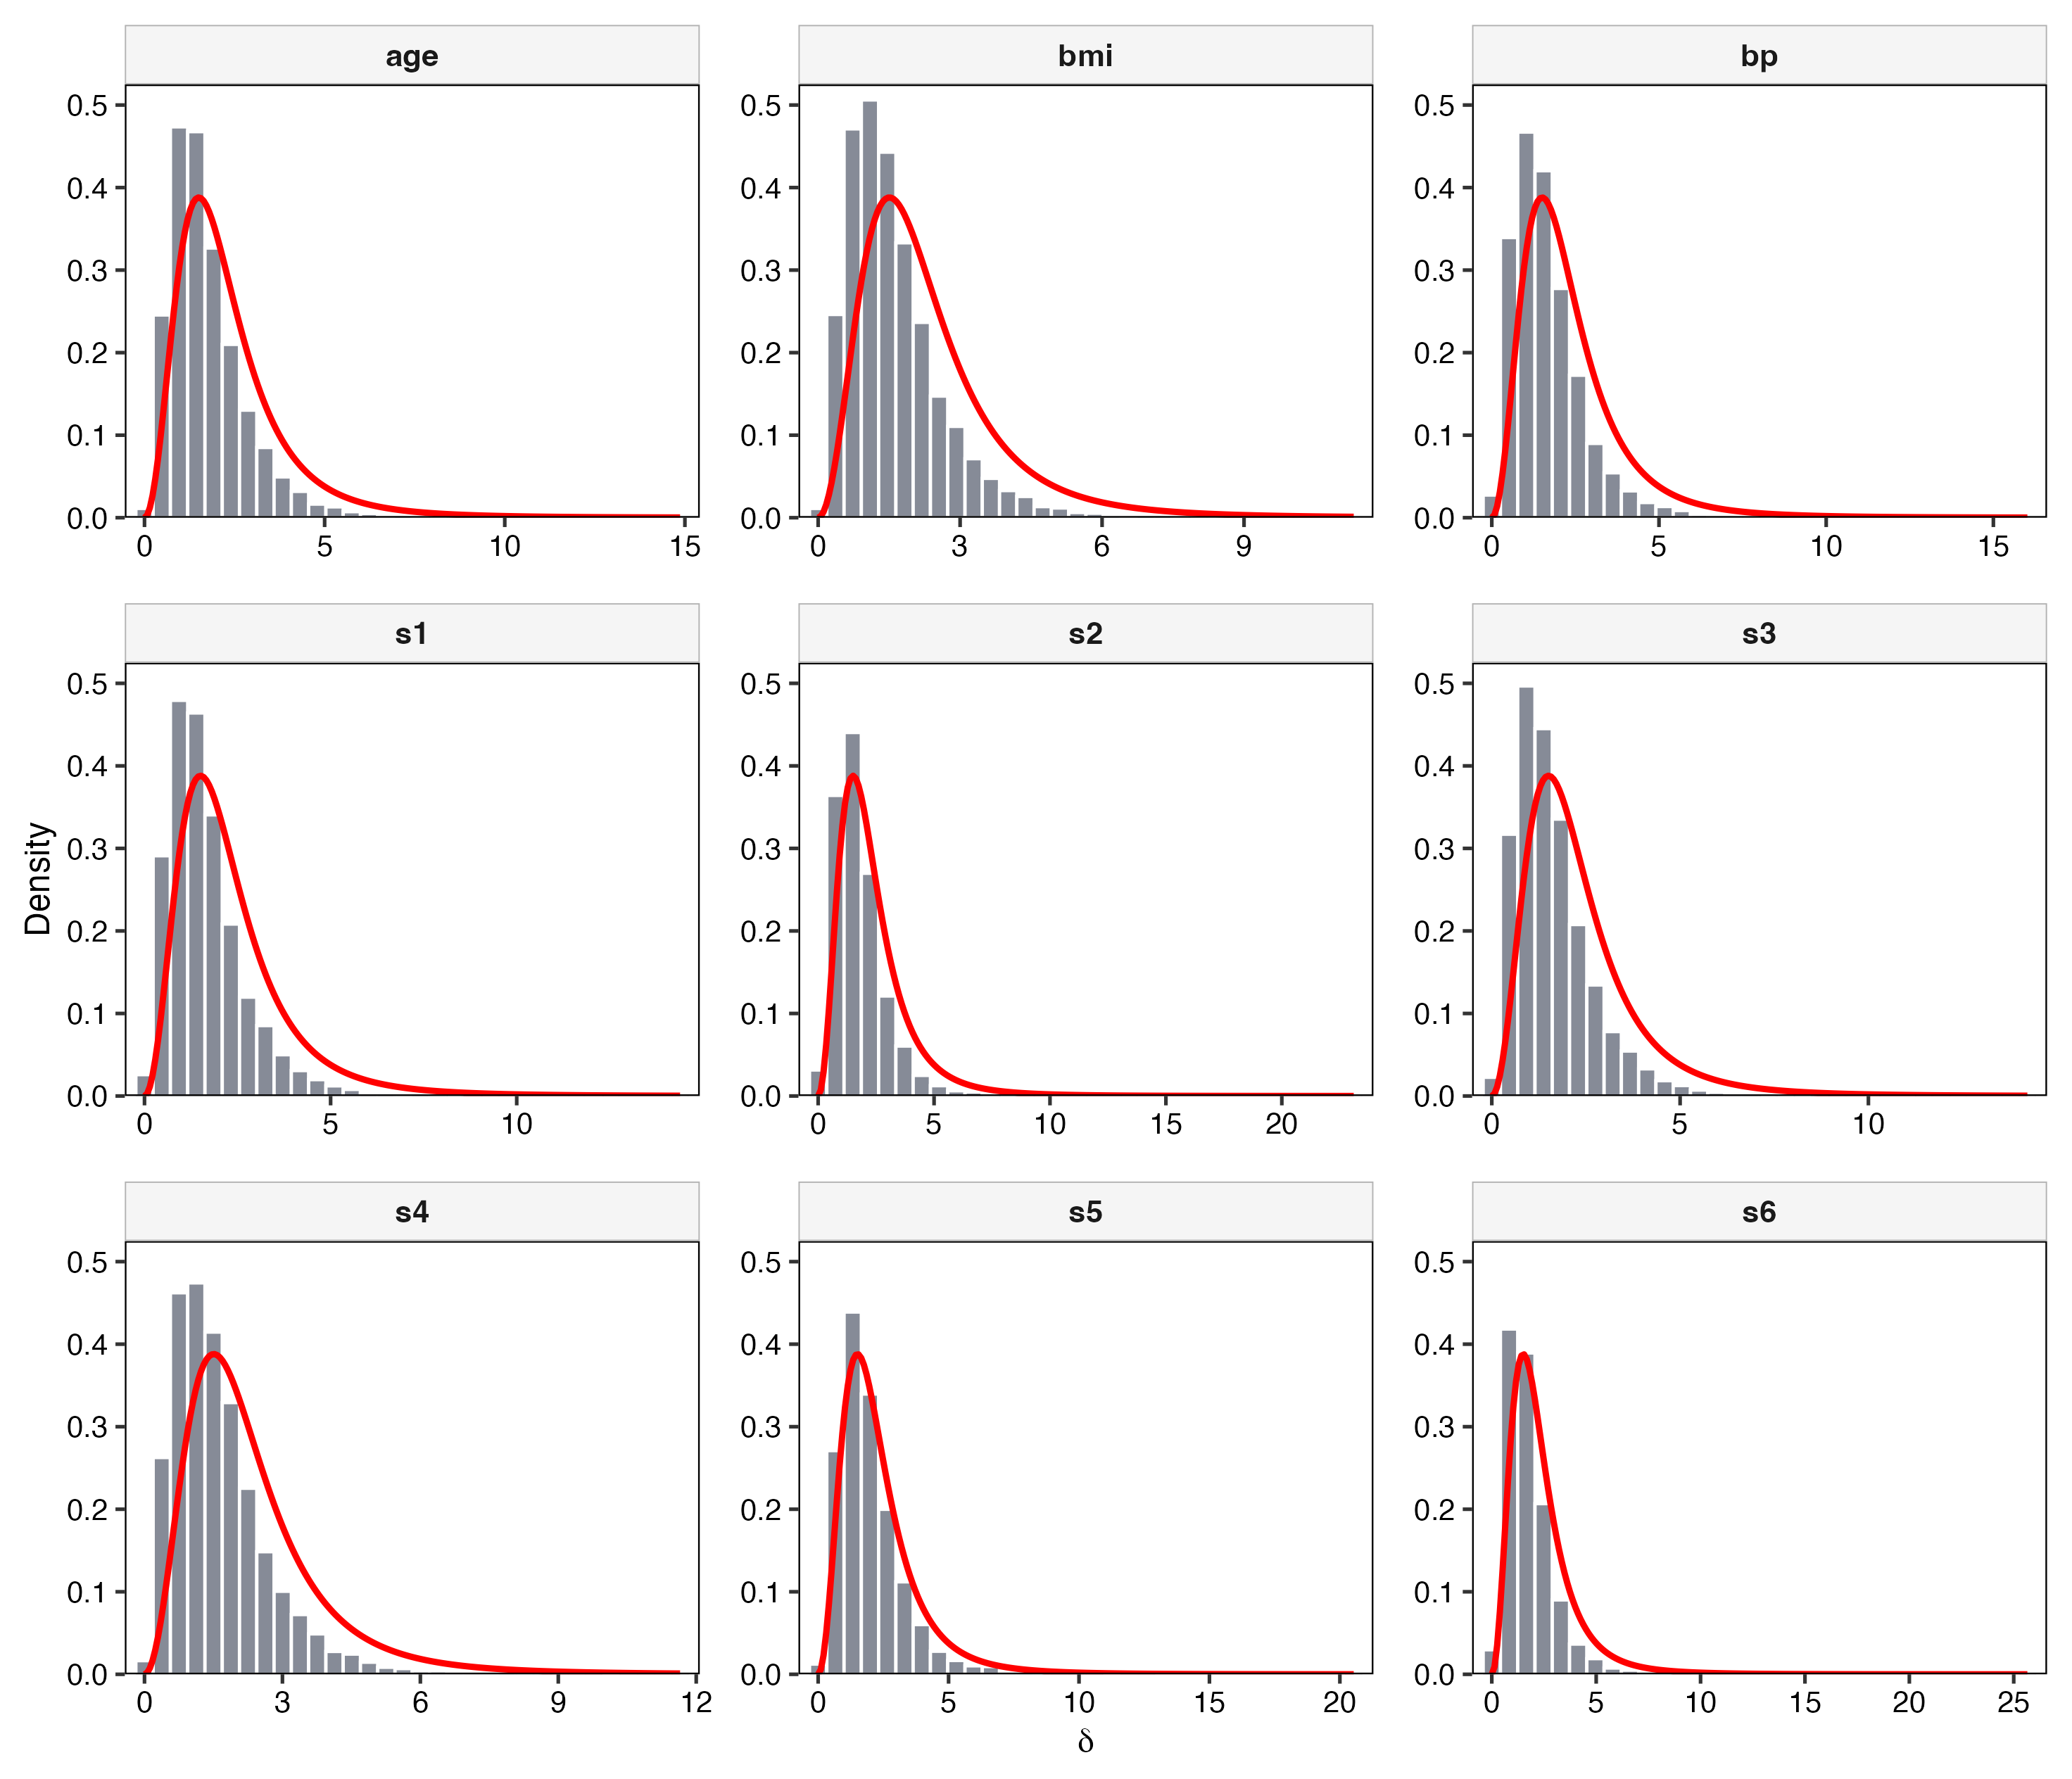
\includegraphics[width=\textwidth]{images/plot-a3-post-delta.png}
  \caption{Diabetes dataset. Marginal posterior distributions of the
    nonlinear magnitude $\delta_j$ for each predictor (grey
    histograms), with the prior density overlaid in red. Across all
    predictors the posterior mass concentrates on small values of
    $\delta_j$ and largely coincides with the prior, consistent with
    the absence of pronounced nonlinear effects reported in
    Section~\ref{sec:empirical}.}
  \label{fig:post-a3-delta}
\end{figure}

\begin{figure}[ht]
  \centering
  
\includegraphics[width=\textwidth]{images/plot-a3-post-theta.png}
  \caption{Diabetes dataset. Marginal posterior distributions of the
    linear coefficient $\theta_j$ for each predictor (grey
    histograms), with the prior density overlaid in red and the null
    value $\theta_j = 0$ marked by the dashed vertical line. The
    posteriors for \texttt{bmi}, \texttt{bp}, and \texttt{s5}
    concentrate well away from zero, whereas the remaining predictors
    place substantial mass near the null.}
  \label{fig:post-a3-theta}
\end{figure}

\begin{figure}[ht]
  \centering
  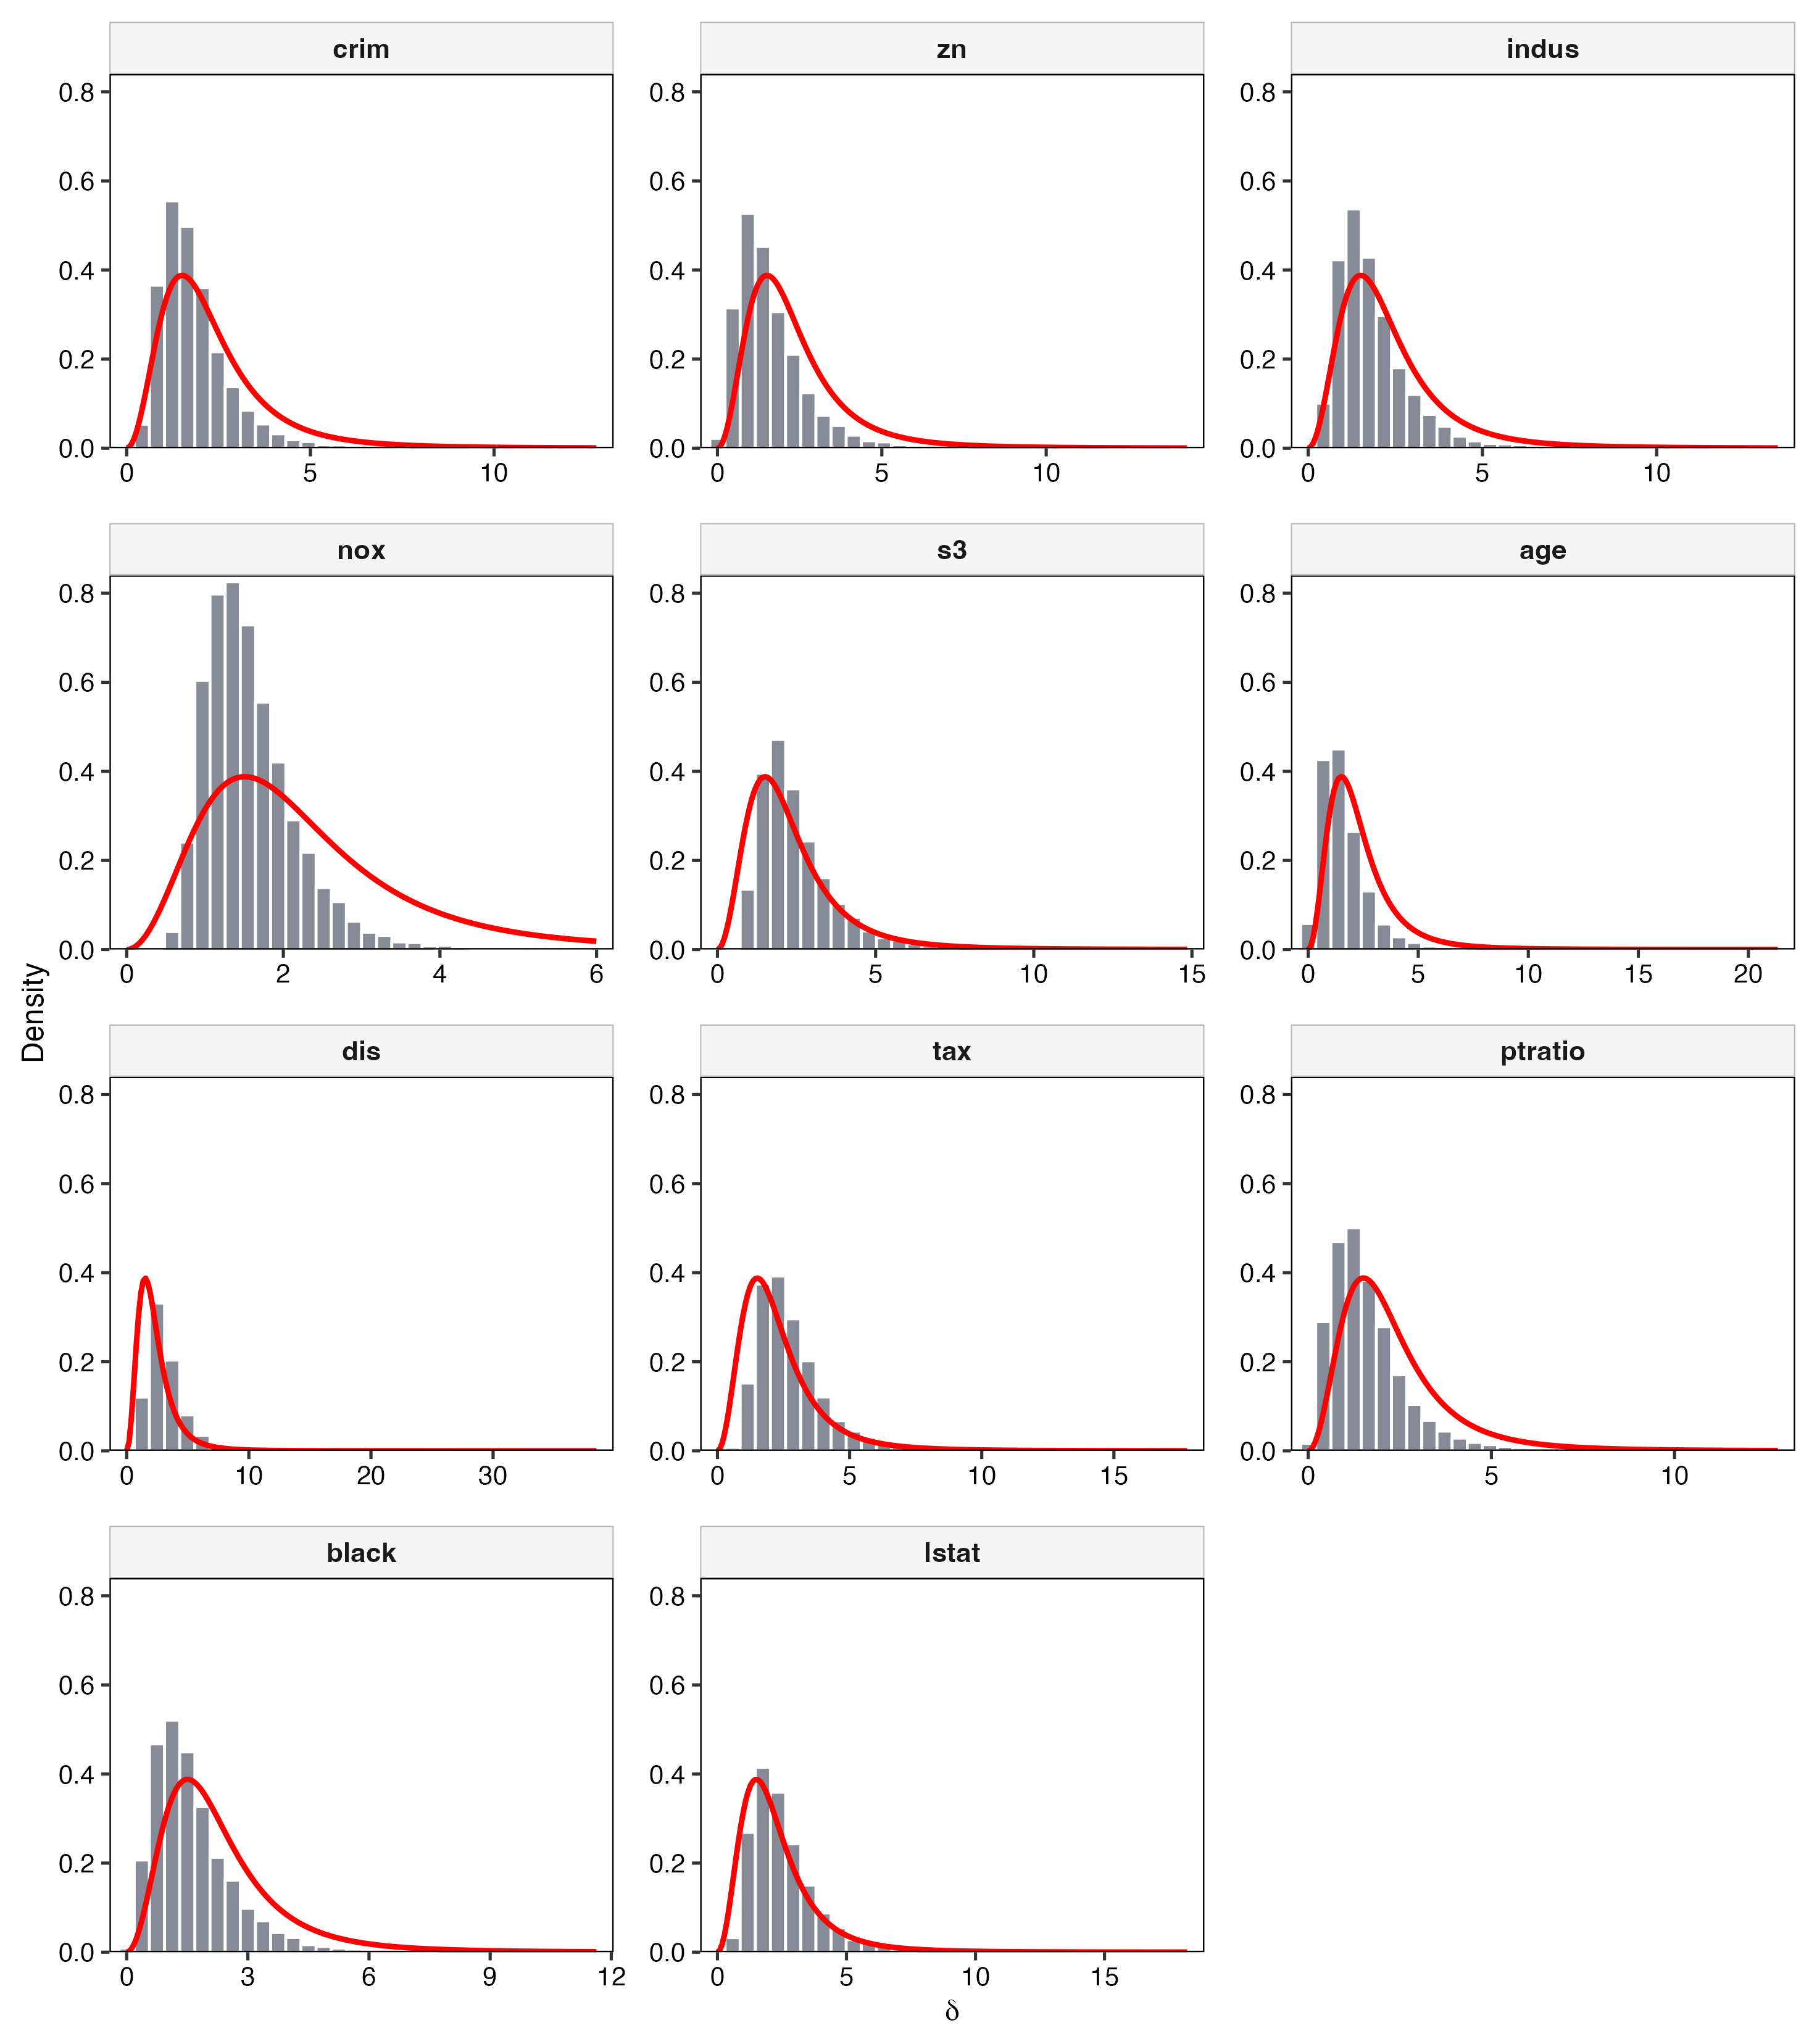
\includegraphics[width=\textwidth]{images/plot-a4-post-delta.png}
  \caption{Boston housing dataset. Marginal posterior distributions of
    the nonlinear magnitude $\delta_j$ for each predictor (grey
    histograms), with the prior density overlaid in red. Most
    predictors show posteriors concentrated at small $\delta_j$; the
    posterior for \texttt{nox} is shifted furthest from the prior,
    consistent with the stronger nonlinear support for that predictor.}
  \label{fig:post-a4-delta}
\end{figure}

\begin{figure}[ht]
  \centering
  
\includegraphics[width=\textwidth]{images/plot-a4-post-theta.png}
  \caption{Boston housing dataset. Marginal posterior distributions of
    the linear coefficient $\theta_j$ for each predictor (grey
    histograms), with the prior density overlaid in red and the null
    value $\theta_j = 0$ marked by the dashed vertical line. Predictors
    such as \texttt{dis}, \texttt{lstat}, \texttt{nox}, and
    \texttt{ptratio} place their posterior mass firmly away from zero,
    reflecting strong linear effects.}
  \label{fig:post-a4-theta}
\end{figure}

\newpage

\printbibliography

\end{document}
